% Options for packages loaded elsewhere
\PassOptionsToPackage{unicode}{hyperref}
\PassOptionsToPackage{hyphens}{url}
%
\documentclass[
]{article}
\usepackage{amsmath,amssymb}
\usepackage{lmodern}
\usepackage{iftex}
\ifPDFTeX
  \usepackage[T1]{fontenc}
  \usepackage[utf8]{inputenc}
  \usepackage{textcomp} % provide euro and other symbols
\else % if luatex or xetex
  \usepackage{unicode-math}
  \defaultfontfeatures{Scale=MatchLowercase}
  \defaultfontfeatures[\rmfamily]{Ligatures=TeX,Scale=1}
\fi
% Use upquote if available, for straight quotes in verbatim environments
\IfFileExists{upquote.sty}{\usepackage{upquote}}{}
\IfFileExists{microtype.sty}{% use microtype if available
  \usepackage[]{microtype}
  \UseMicrotypeSet[protrusion]{basicmath} % disable protrusion for tt fonts
}{}
\makeatletter
\@ifundefined{KOMAClassName}{% if non-KOMA class
  \IfFileExists{parskip.sty}{%
    \usepackage{parskip}
  }{% else
    \setlength{\parindent}{0pt}
    \setlength{\parskip}{6pt plus 2pt minus 1pt}}
}{% if KOMA class
  \KOMAoptions{parskip=half}}
\makeatother
\usepackage{xcolor}
\usepackage[margin=1in]{geometry}
\usepackage{color}
\usepackage{fancyvrb}
\newcommand{\VerbBar}{|}
\newcommand{\VERB}{\Verb[commandchars=\\\{\}]}
\DefineVerbatimEnvironment{Highlighting}{Verbatim}{commandchars=\\\{\}}
% Add ',fontsize=\small' for more characters per line
\usepackage{framed}
\definecolor{shadecolor}{RGB}{248,248,248}
\newenvironment{Shaded}{\begin{snugshade}}{\end{snugshade}}
\newcommand{\AlertTok}[1]{\textcolor[rgb]{0.94,0.16,0.16}{#1}}
\newcommand{\AnnotationTok}[1]{\textcolor[rgb]{0.56,0.35,0.01}{\textbf{\textit{#1}}}}
\newcommand{\AttributeTok}[1]{\textcolor[rgb]{0.77,0.63,0.00}{#1}}
\newcommand{\BaseNTok}[1]{\textcolor[rgb]{0.00,0.00,0.81}{#1}}
\newcommand{\BuiltInTok}[1]{#1}
\newcommand{\CharTok}[1]{\textcolor[rgb]{0.31,0.60,0.02}{#1}}
\newcommand{\CommentTok}[1]{\textcolor[rgb]{0.56,0.35,0.01}{\textit{#1}}}
\newcommand{\CommentVarTok}[1]{\textcolor[rgb]{0.56,0.35,0.01}{\textbf{\textit{#1}}}}
\newcommand{\ConstantTok}[1]{\textcolor[rgb]{0.00,0.00,0.00}{#1}}
\newcommand{\ControlFlowTok}[1]{\textcolor[rgb]{0.13,0.29,0.53}{\textbf{#1}}}
\newcommand{\DataTypeTok}[1]{\textcolor[rgb]{0.13,0.29,0.53}{#1}}
\newcommand{\DecValTok}[1]{\textcolor[rgb]{0.00,0.00,0.81}{#1}}
\newcommand{\DocumentationTok}[1]{\textcolor[rgb]{0.56,0.35,0.01}{\textbf{\textit{#1}}}}
\newcommand{\ErrorTok}[1]{\textcolor[rgb]{0.64,0.00,0.00}{\textbf{#1}}}
\newcommand{\ExtensionTok}[1]{#1}
\newcommand{\FloatTok}[1]{\textcolor[rgb]{0.00,0.00,0.81}{#1}}
\newcommand{\FunctionTok}[1]{\textcolor[rgb]{0.00,0.00,0.00}{#1}}
\newcommand{\ImportTok}[1]{#1}
\newcommand{\InformationTok}[1]{\textcolor[rgb]{0.56,0.35,0.01}{\textbf{\textit{#1}}}}
\newcommand{\KeywordTok}[1]{\textcolor[rgb]{0.13,0.29,0.53}{\textbf{#1}}}
\newcommand{\NormalTok}[1]{#1}
\newcommand{\OperatorTok}[1]{\textcolor[rgb]{0.81,0.36,0.00}{\textbf{#1}}}
\newcommand{\OtherTok}[1]{\textcolor[rgb]{0.56,0.35,0.01}{#1}}
\newcommand{\PreprocessorTok}[1]{\textcolor[rgb]{0.56,0.35,0.01}{\textit{#1}}}
\newcommand{\RegionMarkerTok}[1]{#1}
\newcommand{\SpecialCharTok}[1]{\textcolor[rgb]{0.00,0.00,0.00}{#1}}
\newcommand{\SpecialStringTok}[1]{\textcolor[rgb]{0.31,0.60,0.02}{#1}}
\newcommand{\StringTok}[1]{\textcolor[rgb]{0.31,0.60,0.02}{#1}}
\newcommand{\VariableTok}[1]{\textcolor[rgb]{0.00,0.00,0.00}{#1}}
\newcommand{\VerbatimStringTok}[1]{\textcolor[rgb]{0.31,0.60,0.02}{#1}}
\newcommand{\WarningTok}[1]{\textcolor[rgb]{0.56,0.35,0.01}{\textbf{\textit{#1}}}}
\usepackage{longtable,booktabs,array}
\usepackage{calc} % for calculating minipage widths
% Correct order of tables after \paragraph or \subparagraph
\usepackage{etoolbox}
\makeatletter
\patchcmd\longtable{\par}{\if@noskipsec\mbox{}\fi\par}{}{}
\makeatother
% Allow footnotes in longtable head/foot
\IfFileExists{footnotehyper.sty}{\usepackage{footnotehyper}}{\usepackage{footnote}}
\makesavenoteenv{longtable}
\usepackage{graphicx}
\makeatletter
\def\maxwidth{\ifdim\Gin@nat@width>\linewidth\linewidth\else\Gin@nat@width\fi}
\def\maxheight{\ifdim\Gin@nat@height>\textheight\textheight\else\Gin@nat@height\fi}
\makeatother
% Scale images if necessary, so that they will not overflow the page
% margins by default, and it is still possible to overwrite the defaults
% using explicit options in \includegraphics[width, height, ...]{}
\setkeys{Gin}{width=\maxwidth,height=\maxheight,keepaspectratio}
% Set default figure placement to htbp
\makeatletter
\def\fps@figure{htbp}
\makeatother
\setlength{\emergencystretch}{3em} % prevent overfull lines
\providecommand{\tightlist}{%
  \setlength{\itemsep}{0pt}\setlength{\parskip}{0pt}}
\setcounter{secnumdepth}{-\maxdimen} % remove section numbering
\ifLuaTeX
  \usepackage{selnolig}  % disable illegal ligatures
\fi
\IfFileExists{bookmark.sty}{\usepackage{bookmark}}{\usepackage{hyperref}}
\IfFileExists{xurl.sty}{\usepackage{xurl}}{} % add URL line breaks if available
\urlstyle{same} % disable monospaced font for URLs
\hypersetup{
  pdftitle={Proyect},
  pdfauthor={Cristopher Barrios, Elean Rivas, Angel Higueros, Mariana David},
  hidelinks,
  pdfcreator={LaTeX via pandoc}}

\title{Proyect}
\author{Cristopher Barrios, Elean Rivas, Angel Higueros, Mariana David}
\date{16/2/2023}

\begin{document}
\maketitle

librerias

\begin{verbatim}
## 
## Attaching package: 'dplyr'
\end{verbatim}

\begin{verbatim}
## The following objects are masked from 'package:stats':
## 
##     filter, lag
\end{verbatim}

\begin{verbatim}
## The following objects are masked from 'package:base':
## 
##     intersect, setdiff, setequal, union
\end{verbatim}

\begin{verbatim}
## Warning: package 'ggplot2' was built under R version 4.2.3
\end{verbatim}

\begin{verbatim}
## Package 'mclust' version 6.0.0
## Type 'citation("mclust")' for citing this R package in publications.
\end{verbatim}

\begin{verbatim}
## Welcome! Want to learn more? See two factoextra-related books at https://goo.gl/ve3WBa
\end{verbatim}

\begin{verbatim}
## Warning: package 'GGally' was built under R version 4.2.3
\end{verbatim}

\begin{verbatim}
## Registered S3 method overwritten by 'GGally':
##   method from   
##   +.gg   ggplot2
\end{verbatim}

\begin{verbatim}
## Warning: package 'FeatureImpCluster' was built under R version 4.2.3
\end{verbatim}

\begin{verbatim}
## Loading required package: data.table
\end{verbatim}

\begin{verbatim}
## 
## Attaching package: 'data.table'
\end{verbatim}

\begin{verbatim}
## The following objects are masked from 'package:dplyr':
## 
##     between, first, last
\end{verbatim}

\begin{verbatim}
## Warning: package 'pheatmap' was built under R version 4.2.3
\end{verbatim}

datos

\begin{Shaded}
\begin{Highlighting}[]
\NormalTok{M2009 }\OtherTok{\textless{}{-}} \FunctionTok{read\_sav}\NormalTok{(}\StringTok{"Matrimonios/Matrimonio2009.sav"}\NormalTok{) }\CommentTok{\# nolint}
\NormalTok{M2010 }\OtherTok{\textless{}{-}} \FunctionTok{read\_sav}\NormalTok{(}\StringTok{"Matrimonios/Matrimonio2010.sav"}\NormalTok{) }\CommentTok{\# nolint}
\NormalTok{M2011 }\OtherTok{\textless{}{-}} \FunctionTok{read\_sav}\NormalTok{(}\StringTok{"Matrimonios/Matrimonio2011.sav"}\NormalTok{) }\CommentTok{\# nolint}
\NormalTok{M2012 }\OtherTok{\textless{}{-}} \FunctionTok{read\_sav}\NormalTok{(}\StringTok{"Matrimonios/Matrimonio2012.sav"}\NormalTok{) }\CommentTok{\# nolint}
\NormalTok{M2013 }\OtherTok{\textless{}{-}} \FunctionTok{read\_sav}\NormalTok{(}\StringTok{"Matrimonios/Matrimonio2013.sav"}\NormalTok{) }\CommentTok{\# nolint}
\NormalTok{M2014 }\OtherTok{\textless{}{-}} \FunctionTok{read\_sav}\NormalTok{(}\StringTok{"Matrimonios/Matrimonio2014.sav"}\NormalTok{) }\CommentTok{\# nolint}
\NormalTok{M2015 }\OtherTok{\textless{}{-}} \FunctionTok{read\_sav}\NormalTok{(}\StringTok{"Matrimonios/Matrimonio2015.sav"}\NormalTok{) }\CommentTok{\# nolint}
\NormalTok{M2016 }\OtherTok{\textless{}{-}} \FunctionTok{read\_sav}\NormalTok{(}\StringTok{"Matrimonios/Matrimonio2016.sav"}\NormalTok{) }\CommentTok{\# nolint}
\NormalTok{M2017 }\OtherTok{\textless{}{-}} \FunctionTok{read\_sav}\NormalTok{(}\StringTok{"Matrimonios/Matrimonio2017.sav"}\NormalTok{) }\CommentTok{\# nolint}
\NormalTok{M2018 }\OtherTok{\textless{}{-}} \FunctionTok{read\_sav}\NormalTok{(}\StringTok{"Matrimonios/Matrimonio2018.sav"}\NormalTok{) }\CommentTok{\# nolint}
\NormalTok{M2019 }\OtherTok{\textless{}{-}} \FunctionTok{read\_sav}\NormalTok{(}\StringTok{"Matrimonios/Matrimonio2019.sav"}\NormalTok{) }\CommentTok{\# nolint}
\NormalTok{M2020 }\OtherTok{\textless{}{-}} \FunctionTok{read\_sav}\NormalTok{(}\StringTok{"Matrimonios/Matrimonio2020.sav"}\NormalTok{) }\CommentTok{\# nolint}
\NormalTok{M2021 }\OtherTok{\textless{}{-}} \FunctionTok{read\_sav}\NormalTok{(}\StringTok{"Matrimonios/Matrimonio2021.sav"}\NormalTok{) }\CommentTok{\# nolint}
\end{Highlighting}
\end{Shaded}

Nacimiento

\begin{Shaded}
\begin{Highlighting}[]
\NormalTok{N2009 }\OtherTok{\textless{}{-}} \FunctionTok{read\_sav}\NormalTok{(}\StringTok{"Nacimientos/Nacimiento2009.sav"}\NormalTok{) }\CommentTok{\# nolint}
\NormalTok{N2010 }\OtherTok{\textless{}{-}} \FunctionTok{read\_sav}\NormalTok{(}\StringTok{"Nacimientos/Nacimiento2010.sav"}\NormalTok{) }\CommentTok{\# nolint}
\NormalTok{N2011 }\OtherTok{\textless{}{-}} \FunctionTok{read\_sav}\NormalTok{(}\StringTok{"Nacimientos/Nacimiento2011.sav"}\NormalTok{) }\CommentTok{\# nolint}
\NormalTok{N2012 }\OtherTok{\textless{}{-}} \FunctionTok{read\_sav}\NormalTok{(}\StringTok{"Nacimientos/Nacimiento2012.sav"}\NormalTok{) }\CommentTok{\# nolint}
\NormalTok{N2013 }\OtherTok{\textless{}{-}} \FunctionTok{read\_sav}\NormalTok{(}\StringTok{"Nacimientos/Nacimiento2013.sav"}\NormalTok{) }\CommentTok{\# nolint}
\NormalTok{N2014 }\OtherTok{\textless{}{-}} \FunctionTok{read\_sav}\NormalTok{(}\StringTok{"Nacimientos/Nacimiento2014.sav"}\NormalTok{) }\CommentTok{\# nolint}
\NormalTok{N2015 }\OtherTok{\textless{}{-}} \FunctionTok{read\_sav}\NormalTok{(}\StringTok{"Nacimientos/Nacimiento2015.sav"}\NormalTok{) }\CommentTok{\# nolint}
\NormalTok{N2016 }\OtherTok{\textless{}{-}} \FunctionTok{read\_sav}\NormalTok{(}\StringTok{"Nacimientos/Nacimiento2016.sav"}\NormalTok{) }\CommentTok{\# nolint}
\NormalTok{N2017 }\OtherTok{\textless{}{-}} \FunctionTok{read\_sav}\NormalTok{(}\StringTok{"Nacimientos/Nacimiento2017.sav"}\NormalTok{) }\CommentTok{\# nolint}
\NormalTok{N2018 }\OtherTok{\textless{}{-}} \FunctionTok{read\_sav}\NormalTok{(}\StringTok{"Nacimientos/Nacimiento2018.sav"}\NormalTok{) }\CommentTok{\# nolint}
\NormalTok{N2019 }\OtherTok{\textless{}{-}} \FunctionTok{read\_sav}\NormalTok{(}\StringTok{"Nacimientos/Nacimiento2019.sav"}\NormalTok{) }\CommentTok{\# nolint}
\NormalTok{N2020 }\OtherTok{\textless{}{-}} \FunctionTok{read\_sav}\NormalTok{(}\StringTok{"Nacimientos/Nacimiento2020.sav"}\NormalTok{) }\CommentTok{\# nolint}
\NormalTok{N2021 }\OtherTok{\textless{}{-}} \FunctionTok{read\_sav}\NormalTok{(}\StringTok{"Nacimientos/Nacimiento2021.sav"}\NormalTok{) }\CommentTok{\# nolint}
\end{Highlighting}
\end{Shaded}

Divorcios

\begin{Shaded}
\begin{Highlighting}[]
\NormalTok{D2009 }\OtherTok{\textless{}{-}} \FunctionTok{read\_sav}\NormalTok{(}\StringTok{"Divorcios/Divorcio2009.sav"}\NormalTok{) }\CommentTok{\# nolint}
\NormalTok{D2010 }\OtherTok{\textless{}{-}} \FunctionTok{read\_sav}\NormalTok{(}\StringTok{"Divorcios/Divorcio2010.sav"}\NormalTok{) }\CommentTok{\# nolint}
\NormalTok{D2011 }\OtherTok{\textless{}{-}} \FunctionTok{read\_sav}\NormalTok{(}\StringTok{"Divorcios/Divorcio2011.sav"}\NormalTok{) }\CommentTok{\# nolint}
\NormalTok{D2012 }\OtherTok{\textless{}{-}} \FunctionTok{read\_sav}\NormalTok{(}\StringTok{"Divorcios/Divorcio2012.sav"}\NormalTok{) }\CommentTok{\# nolint}
\NormalTok{D2013 }\OtherTok{\textless{}{-}} \FunctionTok{read\_sav}\NormalTok{(}\StringTok{"Divorcios/Divorcio2013.sav"}\NormalTok{) }\CommentTok{\# nolint}
\NormalTok{D2014 }\OtherTok{\textless{}{-}} \FunctionTok{read\_sav}\NormalTok{(}\StringTok{"Divorcios/Divorcio2014.sav"}\NormalTok{) }\CommentTok{\# nolint}
\NormalTok{D2015 }\OtherTok{\textless{}{-}} \FunctionTok{read\_sav}\NormalTok{(}\StringTok{"Divorcios/Divorcio2015.sav"}\NormalTok{) }\CommentTok{\# nolint}
\NormalTok{D2016 }\OtherTok{\textless{}{-}} \FunctionTok{read\_sav}\NormalTok{(}\StringTok{"Divorcios/Divorcio2016.sav"}\NormalTok{) }\CommentTok{\# nolint}
\NormalTok{D2017 }\OtherTok{\textless{}{-}} \FunctionTok{read\_sav}\NormalTok{(}\StringTok{"Divorcios/Divorcio2017.sav"}\NormalTok{) }\CommentTok{\# nolint}
\NormalTok{D2018 }\OtherTok{\textless{}{-}} \FunctionTok{read\_sav}\NormalTok{(}\StringTok{"Divorcios/Divorcio2018.sav"}\NormalTok{) }\CommentTok{\# nolint}
\NormalTok{D2019 }\OtherTok{\textless{}{-}} \FunctionTok{read\_sav}\NormalTok{(}\StringTok{"Divorcios/Divorcio2019.sav"}\NormalTok{) }\CommentTok{\# nolint}
\NormalTok{D2020 }\OtherTok{\textless{}{-}} \FunctionTok{read\_sav}\NormalTok{(}\StringTok{"Divorcios/Divorcio2020.sav"}\NormalTok{) }\CommentTok{\# nolint}
\NormalTok{D2021 }\OtherTok{\textless{}{-}} \FunctionTok{read\_sav}\NormalTok{(}\StringTok{"Divorcios/Divorcio2021.sav"}\NormalTok{) }\CommentTok{\# nolint}
\end{Highlighting}
\end{Shaded}

\hypertarget{descripciuxf3n-variables-y-observaciones}{%
\subsection{Descripción variables y
observaciones}\label{descripciuxf3n-variables-y-observaciones}}

Comience describiendo cuantas variables y observaciones tiene
disponibles, el tipo de cada una de las variables.

Las bases de datos de matrimonios cuentan con diferentes cantidades de
variables,pero las 22 más comunes son: ---Para divorcios--- DEPREG:
cualitativa MUPREG: cualitativa MESREG: cualitativa AÑOREG: cuantitativa
discreta DIAOCU: cuantitativa MESOCU: cualitativa ANOOCU: cuantitativa
discreta DEPOCU: cualitativa MUPOCU: cualitativa EDADHOM: cuantitativa
discreta EDADMUJ: cuantitativa discreta GETHOM: cualitativa GETMUJ:
cualitativa NACHOM: cualitativa NACMUJ: cualitativa OCUHOM: cualitativa
OCUMUJ: cualitativa MEVER: cualitativa ANOVER: cualitativa

\hypertarget{resumen-de-datos}{%
\subsection{Resumen de datos}\label{resumen-de-datos}}

Haga un resumen de las variables numéricas e investigue si siguen una
distribución normal y tablas de frecuencia para las variables
categóricas, escriba lo que vaya encontrando.

\begin{Shaded}
\begin{Highlighting}[]
\CommentTok{\#summary(M2009)}
\CommentTok{\# Crear una lista con los conjuntos de datos}
\NormalTok{datasets }\OtherTok{\textless{}{-}} \FunctionTok{list}\NormalTok{(D2009, D2010, D2011, D2012, D2013, D2014, D2015, D2016, D2017, D2018, D2019, D2020, D2021)}

\CommentTok{\# Crear un bucle for para analizar cada conjunto de datos y obtener los nombres de las variables numéricas}
\ControlFlowTok{for}\NormalTok{ (i }\ControlFlowTok{in} \DecValTok{1}\SpecialCharTok{:}\FunctionTok{length}\NormalTok{(datasets)) \{}
\NormalTok{  vars\_numéricas }\OtherTok{\textless{}{-}} \FunctionTok{sapply}\NormalTok{(datasets[[i]], is.numeric)}
  \FunctionTok{print}\NormalTok{(}\FunctionTok{names}\NormalTok{(vars\_numéricas[vars\_numéricas]))}
\NormalTok{\}}
\end{Highlighting}
\end{Shaded}

\begin{verbatim}
##  [1] "Depreg"  "Mesreg"  "Diaocu"  "Mesocu"  "Depocu"  "Edadhom" "Edadmuj"
##  [8] "Gethom"  "Getmuj"  "Nachom"  "Nacmuj"  "Ocuhom"  "Ocumuj"  "Mever"  
## [15] "Anover" 
##  [1] "depreg"   "mesreg"   "añoreg"   "diaocu"   "mesocu"   "añoocu"  
##  [7] "depocu"   "edadhom"  "edadmuj"  "grethom"  "gretmuj"  "nachom"  
## [13] "nacmuj"   "escohom"  "escomuj"  "ocupahom" "ocupamuj"
##  [1] "depreg"   "mesreg"   "añoreg"   "diaocu"   "mesocu"   "añoocu"  
##  [7] "depocu"   "edadhom"  "edadmuj"  "grethom"  "gretmuj"  "nachom"  
## [13] "nacmuj"   "escohom"  "escomuj"  "ocupahom" "ocupamuj"
##  [1] "DEPREG"  "MESREG"  "AÑOREG"  "DIAOCU"  "MESOCU"  "DEPOCU"  "EDADHOM"
##  [8] "EDADMUJ" "GETHOM"  "GETMUJ"  "NACHOM"  "NACMUJ"  "ESCHOM"  "ESCMUJ" 
##  [1] "DEPREG"  "MESREG"  "AÑOREG"  "DIAOCU"  "MESOCU"  "DEPOCU"  "EDADHOM"
##  [8] "EDADMUJ" "PUEHOM"  "PUEMUJ"  "NACHOM"  "NACMUJ"  "ESCHOM"  "ESCMUJ" 
##  [1] "DEPREG"  "MESREG"  "AÑOREG"  "DIAOCU"  "MESOCU"  "DEPOCU"  "EDADHOM"
##  [8] "EDADMUJ" "PUEHOM"  "PUEMUJ"  "NACHOM"  "NACMUJ"  "ESCHOM"  "ESCMUJ" 
##  [1] "DEPREG"  "MESREG"  "AÑOREG"  "DIAOCU"  "MESOCU"  "AÑOOCU"  "DEPOCU" 
##  [8] "EDADHOM" "EDADMUJ" "PUEHOM"  "PUEMUJ"  "NACHOM"  "NACMUJ"  "ESCHOM" 
## [15] "ESCMUJ"  "CIUOHOM" "CIUOMUJ"
##  [1] "DEPREG"  "MESREG"  "AÑOREG"  "DIAOCU"  "MESOCU"  "AÑOOCU"  "DEPOCU" 
##  [8] "EDADHOM" "EDADMUJ" "PPERHOM" "PPERMUJ" "NACHOM"  "NACMUJ"  "ESCHOM" 
## [15] "ESCMUJ"  "CIUOHOM" "CIUOMUJ"
##  [1] "DEPREG"  "MESREG"  "AÑOREG"  "DIAOCU"  "MESOCU"  "AÑOOCU"  "DEPOCU" 
##  [8] "EDADHOM" "EDADMUJ" "PPERHOM" "PPERMUJ" "NACHOM"  "NACMUJ"  "ESCHOM" 
## [15] "ESCMUJ"  "CIUOHOM" "CIUOMUJ"
##  [1] "DEPREG"  "MESREG"  "AÑOREG"  "DIAOCU"  "MESOCU"  "AÑOOCU"  "DEPOCU" 
##  [8] "EDADHOM" "EDADMUJ" "PPERHOM" "PPERMUJ" "NACHOM"  "NACMUJ"  "ESCHOM" 
## [15] "ESCMUJ"  "CIUOHOM" "CIUOMUJ"
##  [1] "DEPREG"  "MESREG"  "AÑOREG"  "DIAOCU"  "MESOCU"  "AÑOOCU"  "DEPOCU" 
##  [8] "EDADHOM" "EDADMUJ" "PPERHOM" "PPERMUJ" "NACHOM"  "NACMUJ"  "ESCHOM" 
## [15] "ESCMUJ"  "CIUOHOM" "CIUOMUJ"
##  [1] "DEPREG"  "MESREG"  "AÑOREG"  "DIAOCU"  "MESOCU"  "AÑOOCU"  "DEPOCU" 
##  [8] "EDADHOM" "EDADMUJ" "PPERHOM" "PPERMUJ" "NACHOM"  "NACMUJ"  "ESCHOM" 
## [15] "ESCMUJ"  "CIUOHOM" "CIUOMUJ"
##  [1] "DEPREG"  "MESREG"  "AÑOREG"  "DIAOCU"  "MESOCU"  "AÑOOCU"  "DEPOCU" 
##  [8] "EDADHOM" "EDADMUJ" "PPERHOM" "PPERMUJ" "NACHOM"  "NACMUJ"  "ESCHOM" 
## [15] "ESCMUJ"
\end{verbatim}

\hypertarget{variables-importantes}{%
\subsection{Variables importantes}\label{variables-importantes}}

Cruce las variables que considere que son las más importantes para
hallar los elementos clave que lo pueden llevar a comprender lo que está
causando el problema encontrado.

Tiempo: Es importante poder ver el cambio a través del tiempo, si ha
habido un incremente o decremento, tanto en matrimonios como en
divorcios

NUNUHO:``Número de nupcias del hombre'' NUNUMU:``Número de nupcias de la
mujer''

\begin{Shaded}
\begin{Highlighting}[]
\NormalTok{M2021[, }\FunctionTok{c}\NormalTok{(}\DecValTok{7}\NormalTok{, }\DecValTok{8}\NormalTok{)]}
\end{Highlighting}
\end{Shaded}

\begin{verbatim}
## # A tibble: 87,480 x 2
##    NUNUHO       NUNUMU      
##    <dbl+lbl>    <dbl+lbl>   
##  1 9 [Ignorado] 9 [Ignorado]
##  2 1            1           
##  3 9 [Ignorado] 9 [Ignorado]
##  4 1            1           
##  5 9 [Ignorado] 9 [Ignorado]
##  6 9 [Ignorado] 9 [Ignorado]
##  7 9 [Ignorado] 9 [Ignorado]
##  8 1            1           
##  9 9 [Ignorado] 9 [Ignorado]
## 10 9 [Ignorado] 9 [Ignorado]
## # ... with 87,470 more rows
\end{verbatim}

Saber si una persona ha estado previamente casada y si esto influye en
la posibilidad de divorcio, cómo hipotesis se espera que las personas
que han tenido más de dos nupcias antes, son más propensas al divorcio

Edadhom: ``Edad del hombre'' Edadmuj: ``Edad de la mujer''

\begin{Shaded}
\begin{Highlighting}[]
\NormalTok{D2021[, }\FunctionTok{c}\NormalTok{(}\DecValTok{10}\NormalTok{, }\DecValTok{11}\NormalTok{)]}
\end{Highlighting}
\end{Shaded}

\begin{verbatim}
## # A tibble: 9,621 x 2
##    EDADHOM        EDADMUJ       
##    <dbl+lbl>      <dbl+lbl>     
##  1  29             25           
##  2  36             37           
##  3  34             31           
##  4  48             33           
##  5  44             28           
##  6  39             27           
##  7  45             40           
##  8 999 [Ignorado] 999 [Ignorado]
##  9  36             31           
## 10 999 [Ignorado] 999 [Ignorado]
## # ... with 9,611 more rows
\end{verbatim}

La edad puede ser un dato interesante a explorar, esto para saber si los
jovenes tienen más tendencia a casarse o divorcioarse y si los
matrimonios más duraderos tienen menos divorcios

Genero: Es interesante ver que genero es más propenso a los divorcios,
esto también puede estar relacionado con la cantidad de nupcias de una
persona

Efectos de la pandemia: Ver como los divorcios y matrimonios se
comportaron a partir de marzo de 2020 que fue el momento en que la
cuarentena empezó a hacerse efectiva

\hypertarget{graficos-exploratorios}{%
\subsection{Graficos exploratorios}\label{graficos-exploratorios}}

Haga gráficos exploratorios que le de ideas del estado de los datos.

\begin{longtable}[]{@{}
  >{\raggedright\arraybackslash}p{(\columnwidth - 0\tabcolsep) * \real{1.0000}}@{}}
\toprule()
\endhead
\#\# Analisis \\
\#\# Divorcios \\
\texttt{r\ EdadMujD2009\ \textless{}-\ sum(D2009\$Edadmuj)\ EdadMujD2010\ \textless{}-\ sum(D2010\$edadmuj)\ EdadMujD2011\ \textless{}-\ sum(D2011\$edadmuj)\ EdadMujD2012\ \textless{}-\ sum(D2012\$EDADMUJ)\ EdadMujD2013\ \textless{}-\ sum(D2013\$EDADMUJ)\ EdadMujD2014\ \textless{}-\ sum(D2014\$EDADMUJ)\ EdadMujD2015\ \textless{}-\ sum(D2015\$EDADMUJ)\ EdadMujD2016\ \textless{}-\ sum(D2016\$EDADMUJ)\ EdadMujD2017\ \textless{}-\ sum(D2017\$EDADMUJ)\ EdadMujD2018\ \textless{}-\ sum(D2018\$EDADMUJ)\ EdadMujD2019\ \textless{}-\ sum(D2019\$EDADMUJ)\ EdadMujD2020\ \textless{}-\ sum(D2020\$EDADMUJ)\ EdadMujD2021\ \textless{}-\ sum(D2021\$EDADMUJ)} \\
\texttt{r\ dfD\ \textless{}-\ data.frame\ (año\ \ =\ c("2009",\ "2010",\ "2011",\ "2012",\ "2013",\ "2014",\ "2015",\ "2016",\ "2017","2018","2019","2020","2021"),\ matrimonios\ =\ c(EdadMujD2009,\ EdadMujD2010,\ EdadMujD2011,\ EdadMujD2012,\ EdadMujD2013,\ EdadMujD2014,\ EdadMujD2015,\ EdadMujD2016,\ EdadMujD2017,\ EdadMujD2018,\ EdadMujD2019,\ EdadMujD2020,\ EdadMujD2021))\ print(dfD)} \\
\texttt{\#\#\ \ \ \ \ año\ matrimonios\ \#\#\ 1\ \ 2009\ \ \ \ \ 1173016\ \#\#\ 2\ \ 2010\ \ \ \ \ 2764309\ \#\#\ 3\ \ 2011\ \ \ \ \ 3086834\ \#\#\ 4\ \ 2012\ \ \ \ \ 3512781\ \#\#\ 5\ \ 2013\ \ \ \ \ 3572498\ \#\#\ 6\ \ 2014\ \ \ \ \ 3342987\ \#\#\ 7\ \ 2015\ \ \ \ \ 3251831\ \#\#\ 8\ \ 2016\ \ \ \ \ 3064039\ \#\#\ 9\ \ 2017\ \ \ \ \ 3042894\ \#\#\ 10\ 2018\ \ \ \ \ 3062850\ \#\#\ 11\ 2019\ \ \ \ \ 3933259\ \#\#\ 12\ 2020\ \ \ \ \ 1687235\ \#\#\ 13\ 2021\ \ \ \ \ 3733294} \\
\texttt{r\ ggplot(dfD,\ aes(x=año,\ y=matrimonios,\ group\ =\ 1))\ +\ geom\_point(size\ =\ 2,\ color\ =\ "green")\ +\ geom\_line(color="green")\ +\ labs(x\ =\ "Año",\ y\ =\ "Divorcios",\ title\ =\ "Divorcios")} \\
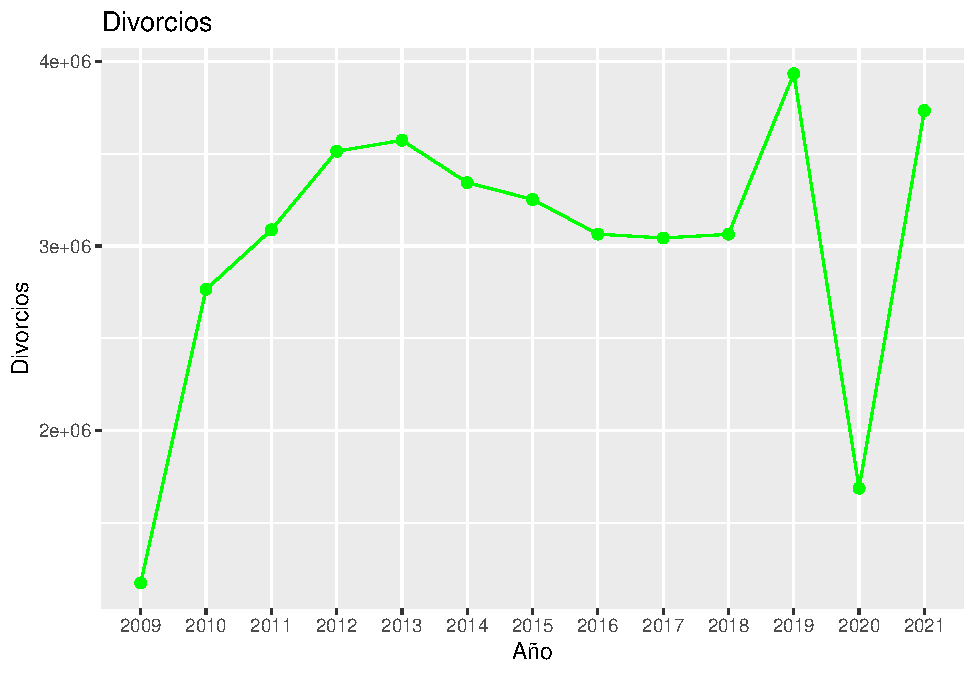
\includegraphics{Proyecto_files/figure-latex/unnamed-chunk-10-1.pdf} \\
\#\# Matrimonios \\
\texttt{r\ EdadMujM2009\ \textless{}-\ sum(M2009\$Edadmuj)} \\
\texttt{\#\#\ Warning:\ Unknown\ or\ uninitialised\ column:\ \textasciigrave{}Edadmuj\textasciigrave{}.} \\
\texttt{r\ EdadMujM2010\ \textless{}-\ sum(M2010\$edadmuj)} \\
\texttt{\#\#\ Warning:\ Unknown\ or\ uninitialised\ column:\ \textasciigrave{}edadmuj\textasciigrave{}.} \\
\texttt{r\ EdadMujM2011\ \textless{}-\ sum(M2011\$edadmuj)} \\
\texttt{\#\#\ Warning:\ Unknown\ or\ uninitialised\ column:\ \textasciigrave{}edadmuj\textasciigrave{}.} \\
\texttt{r\ EdadMujM2012\ \textless{}-\ sum(M2012\$EDADMUJ)\ EdadMujM2013\ \textless{}-\ sum(M2013\$EDADMUJ)\ EdadMujM2014\ \textless{}-\ sum(M2014\$EDADMUJ)\ EdadMujM2015\ \textless{}-\ sum(M2015\$EDADMUJ)\ EdadMujM2016\ \textless{}-\ sum(M2016\$EDADMUJ)\ EdadMujM2017\ \textless{}-\ sum(M2017\$EDADMUJ)\ EdadMujM2018\ \textless{}-\ sum(M2018\$EDADMUJ)\ EdadMujM2019\ \textless{}-\ sum(M2019\$EDADMUJ)\ EdadMujM2020\ \textless{}-\ sum(M2020\$EDADMUJ)\ EdadMujM2021\ \textless{}-\ sum(M2021\$EDADMUJ)} \\
\texttt{r\ dfD\ \textless{}-\ data.frame\ (año\ \ =\ c("2009",\ "2010",\ "2011",\ "2012",\ "2013",\ "2014",\ "2015",\ "2016",\ "2017","2018","2019","2020","2021"),\ matrimonios\ =\ c(EdadMujM2009,\ EdadMujM2010,\ EdadMujM2011,\ EdadMujM2012,\ EdadMujM2013,\ EdadMujM2014,\ EdadMujM2015,\ EdadMujM2016,\ EdadMujM2017,\ EdadMujM2018,\ EdadMujM2019,\ EdadMujM2020,\ EdadMujM2021))\ print(dfD)} \\
\texttt{\#\#\ \ \ \ \ año\ matrimonios\ \#\#\ 1\ \ 2009\ \ \ \ \ \ \ \ \ \ \ 0\ \#\#\ 2\ \ 2010\ \ \ \ \ \ \ \ \ \ \ 0\ \#\#\ 3\ \ 2011\ \ \ \ \ \ \ \ \ \ \ 0\ \#\#\ 4\ \ 2012\ \ \ \ \ 2251360\ \#\#\ 5\ \ 2013\ \ \ \ \ 2116792\ \#\#\ 6\ \ 2014\ \ \ \ \ 2089815\ \#\#\ 7\ \ 2015\ \ \ \ \ 2065832\ \#\#\ 8\ \ 2016\ \ \ \ \ 1914942\ \#\#\ 9\ \ 2017\ \ \ \ \ 1949642\ \#\#\ 10\ 2018\ \ \ \ \ 2038355\ \#\#\ 11\ 2019\ \ \ \ \ 2094080\ \#\#\ 12\ 2020\ \ \ \ \ 1555747\ \#\#\ 13\ 2021\ \ \ \ \ 2407251} \\
\texttt{r\ ggplot(dfD,\ aes(x=año,\ y=matrimonios,\ group\ =\ 1))\ +\ geom\_point(size\ =\ 2,\ color\ =\ "green")\ +\ geom\_line(color="green")\ +\ labs(x\ =\ "Año",\ y\ =\ "Matrimonios",\ title\ =\ "Matrimonios")} \\
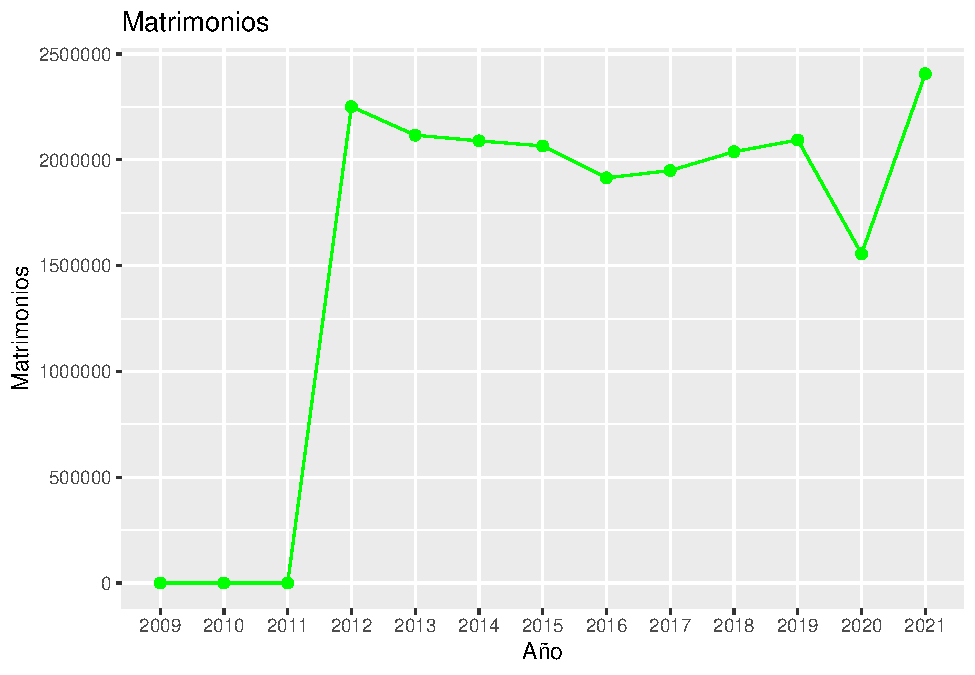
\includegraphics{Proyecto_files/figure-latex/unnamed-chunk-13-1.pdf} \\
\#\# Nacimientos \\
\texttt{r\ EdadMujN2009\ \textless{}-\ sum(N2009\$Edadm)\ EdadMujN2010\ \textless{}-\ sum(N2010\$Edadm)\ EdadMujN2011\ \textless{}-\ sum(N2011\$Edadm)\ EdadMujN2012\ \textless{}-\ sum(N2012\$Edadm)\ EdadMujN2013\ \textless{}-\ sum(N2013\$Edadm)\ EdadMujN2014\ \textless{}-\ sum(N2014\$Edadm)\ EdadMujN2015\ \textless{}-\ sum(N2015\$Edadm)\ EdadMujN2016\ \textless{}-\ sum(N2016\$Edadm)\ EdadMujN2017\ \textless{}-\ sum(N2017\$Edadm)\ EdadMujN2018\ \textless{}-\ sum(N2018\$Edadm)\ EdadMujN2019\ \textless{}-\ sum(N2019\$Edadm)\ EdadMujN2020\ \textless{}-\ sum(N2020\$Edadm)\ EdadMujN2021\ \textless{}-\ sum(N2021\$Edadm)} \\
\texttt{r\ dNac\ \textless{}-\ data.frame\ (año\ \ =\ c("2009",\ "2010",\ "2011",\ "2012",\ "2013",\ "2014",\ "2015",\ "2016",\ "2017","2018","2019","2020","2021"),\ matrimonios\ =\ c(EdadMujN2009,\ EdadMujN2010,\ EdadMujN2011,\ EdadMujN2012,\ EdadMujN2013,\ EdadMujN2014,\ EdadMujN2015,\ EdadMujN2016,\ EdadMujN2017,\ EdadMujN2018,\ EdadMujN2019,\ EdadMujN2020,\ EdadMujN2021))\ print(dNac)} \\
\texttt{\#\#\ \ \ \ \ año\ matrimonios\ \#\#\ 1\ \ 2009\ \ \ \ 20298288\ \#\#\ 2\ \ 2010\ \ \ \ \ 9550498\ \#\#\ 3\ \ 2011\ \ \ \ \ 9713100\ \#\#\ 4\ \ 2012\ \ \ \ \ 9974089\ \#\#\ 5\ \ 2013\ \ \ \ 10152809\ \#\#\ 6\ \ 2014\ \ \ \ 10021535\ \#\#\ 7\ \ 2015\ \ \ \ 10162460\ \#\#\ 8\ \ 2016\ \ \ \ 10093076\ \#\#\ 9\ \ 2017\ \ \ \ \ 9862143\ \#\#\ 10\ 2018\ \ \ \ \ 9922821\ \#\#\ 11\ 2019\ \ \ \ \ 9922821\ \#\#\ 12\ 2020\ \ \ \ \ 9473381\ \#\#\ 13\ 2021\ \ \ \ \ 8949596} \\
\texttt{r\ ggplot(dNac,\ aes(x=año,\ y=matrimonios,\ group\ =\ 1))\ +\ geom\_point(size\ =\ 2,\ color\ =\ "green")\ +\ geom\_line(color="green")\ +\ labs(x\ =\ "Año",\ y\ =\ "Nacimientos",\ title\ =\ "Nacimientos")} \\
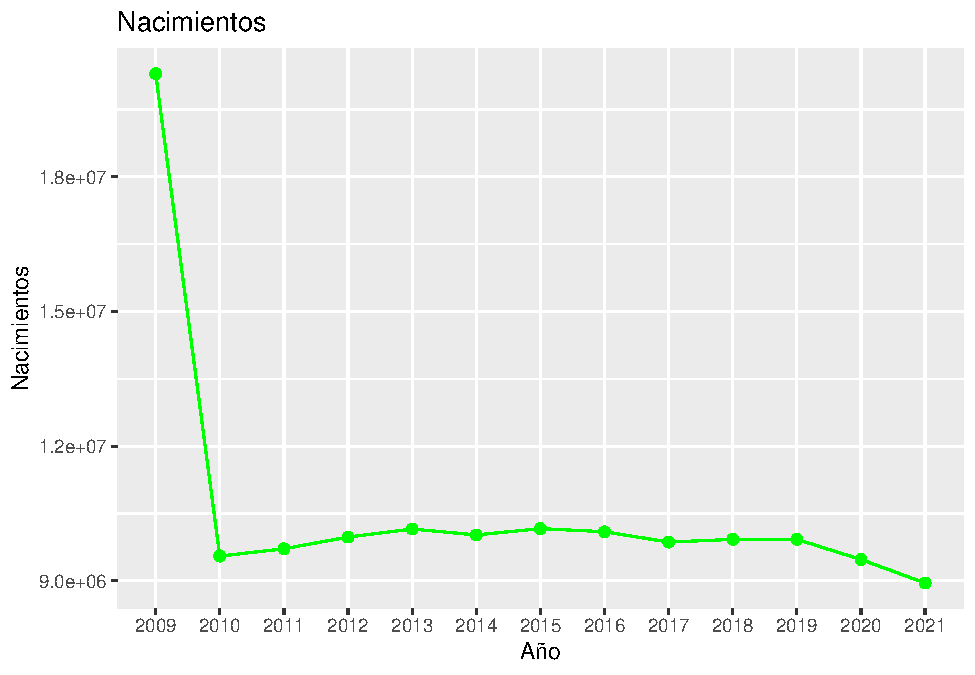
\includegraphics{Proyecto_files/figure-latex/unnamed-chunk-16-1.pdf} \\
\bottomrule()
\end{longtable}

\hypertarget{histogramas}{%
\subsection{Histogramas}\label{histogramas}}

2009

\begin{Shaded}
\begin{Highlighting}[]
\FunctionTok{library}\NormalTok{(dplyr)}
\FunctionTok{library}\NormalTok{(ggplot2)}

\NormalTok{D2009 }\OtherTok{\textless{}{-}} \FunctionTok{subset}\NormalTok{(D2009, Edadmuj }\SpecialCharTok{\textless{}} \DecValTok{999}\NormalTok{)}

\FunctionTok{barplot}\NormalTok{(}\FunctionTok{table}\NormalTok{(D2009}\SpecialCharTok{$}\NormalTok{Edadmuj), }\AttributeTok{main =} \StringTok{"Edad de la mujer en divorcios 2009"}\NormalTok{, }\AttributeTok{xlab =} \StringTok{"Edad"}\NormalTok{, }\AttributeTok{ylab =} \StringTok{"Cantidad"}\NormalTok{, }\AttributeTok{col =} \StringTok{"steelblue"}\NormalTok{ , }\AttributeTok{border =} \StringTok{"pink"}\NormalTok{)}
\end{Highlighting}
\end{Shaded}

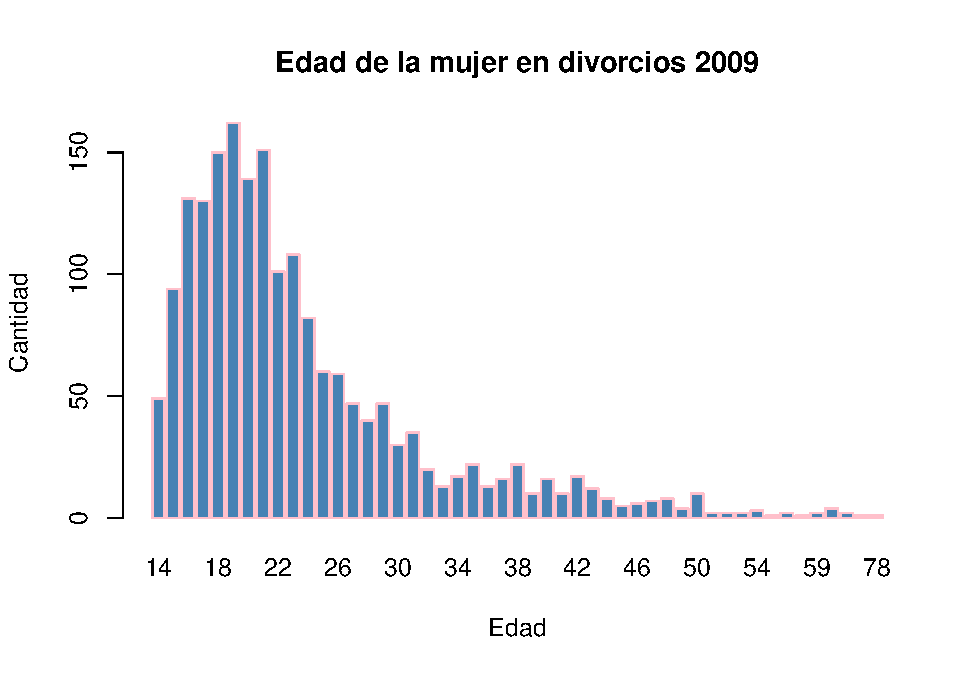
\includegraphics{Proyecto_files/figure-latex/unnamed-chunk-17-1.pdf}

2010

\begin{Shaded}
\begin{Highlighting}[]
\NormalTok{D2010 }\OtherTok{\textless{}{-}} \FunctionTok{subset}\NormalTok{(D2010, edadmuj }\SpecialCharTok{\textless{}} \DecValTok{999}\NormalTok{)}

\FunctionTok{barplot}\NormalTok{(}\FunctionTok{table}\NormalTok{(D2010}\SpecialCharTok{$}\NormalTok{edadmuj), }\AttributeTok{main =} \StringTok{"Edad de la mujer en divorcios 2010"}\NormalTok{, }\AttributeTok{xlab =} \StringTok{"Edad"}\NormalTok{, }\AttributeTok{ylab =} \StringTok{"Cantidad"}\NormalTok{, }\AttributeTok{col =} \StringTok{"steelblue"}\NormalTok{ , }\AttributeTok{border =} \StringTok{"pink"}\NormalTok{)}
\end{Highlighting}
\end{Shaded}

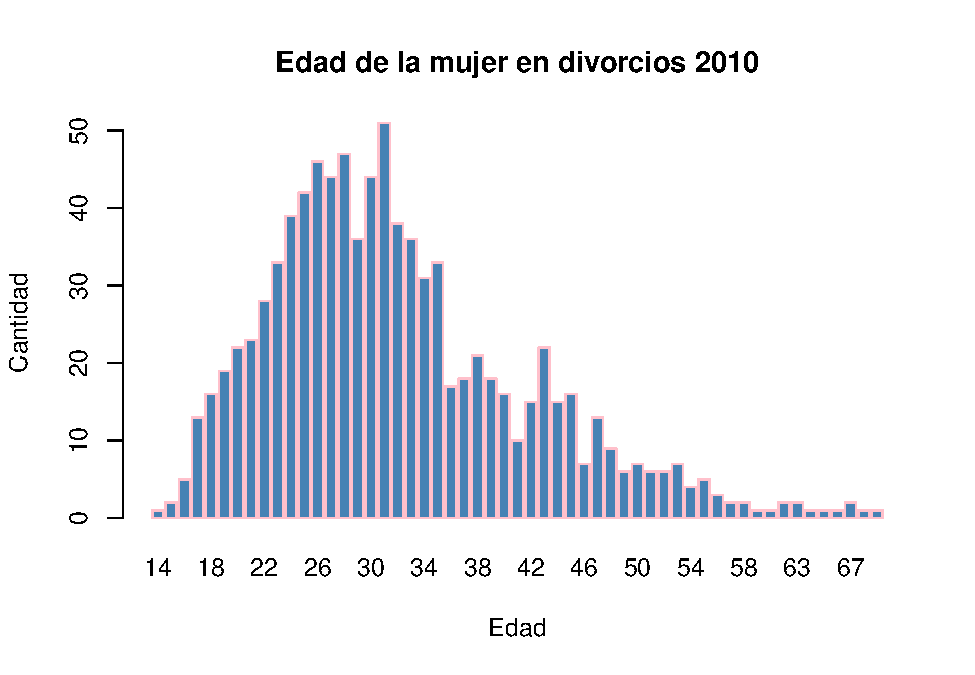
\includegraphics{Proyecto_files/figure-latex/unnamed-chunk-18-1.pdf}

2011

\begin{Shaded}
\begin{Highlighting}[]
\NormalTok{D2011 }\OtherTok{\textless{}{-}} \FunctionTok{subset}\NormalTok{(D2011, edadmuj }\SpecialCharTok{\textless{}} \DecValTok{999}\NormalTok{)}

\FunctionTok{barplot}\NormalTok{(}\FunctionTok{table}\NormalTok{(D2011}\SpecialCharTok{$}\NormalTok{edadmuj), }\AttributeTok{main =} \StringTok{"Edad de la mujer en divorcios 2011"}\NormalTok{, }\AttributeTok{xlab =} \StringTok{"Edad"}\NormalTok{, }\AttributeTok{ylab =} \StringTok{"Cantidad"}\NormalTok{, }\AttributeTok{col =} \StringTok{"steelblue"}\NormalTok{ , }\AttributeTok{border =} \StringTok{"pink"}\NormalTok{)}
\end{Highlighting}
\end{Shaded}

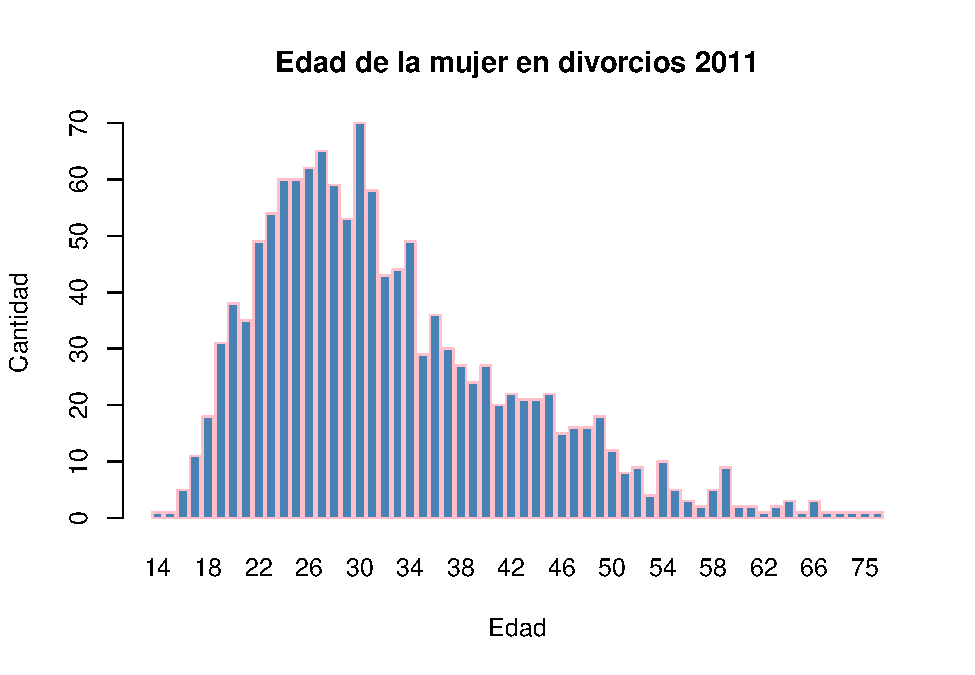
\includegraphics{Proyecto_files/figure-latex/unnamed-chunk-19-1.pdf}

2012

\begin{Shaded}
\begin{Highlighting}[]
\NormalTok{D2012 }\OtherTok{\textless{}{-}} \FunctionTok{subset}\NormalTok{(D2012, EDADMUJ }\SpecialCharTok{\textless{}} \DecValTok{999}\NormalTok{)}

\FunctionTok{barplot}\NormalTok{(}\FunctionTok{table}\NormalTok{(D2012}\SpecialCharTok{$}\NormalTok{EDADMUJ), }\AttributeTok{main =} \StringTok{"Edad de la mujer en divorcios 2012"}\NormalTok{, }\AttributeTok{xlab =} \StringTok{"Edad"}\NormalTok{, }\AttributeTok{ylab =} \StringTok{"Cantidad"}\NormalTok{, }\AttributeTok{col =} \StringTok{"steelblue"}\NormalTok{ , }\AttributeTok{border =} \StringTok{"pink"}\NormalTok{)}
\end{Highlighting}
\end{Shaded}

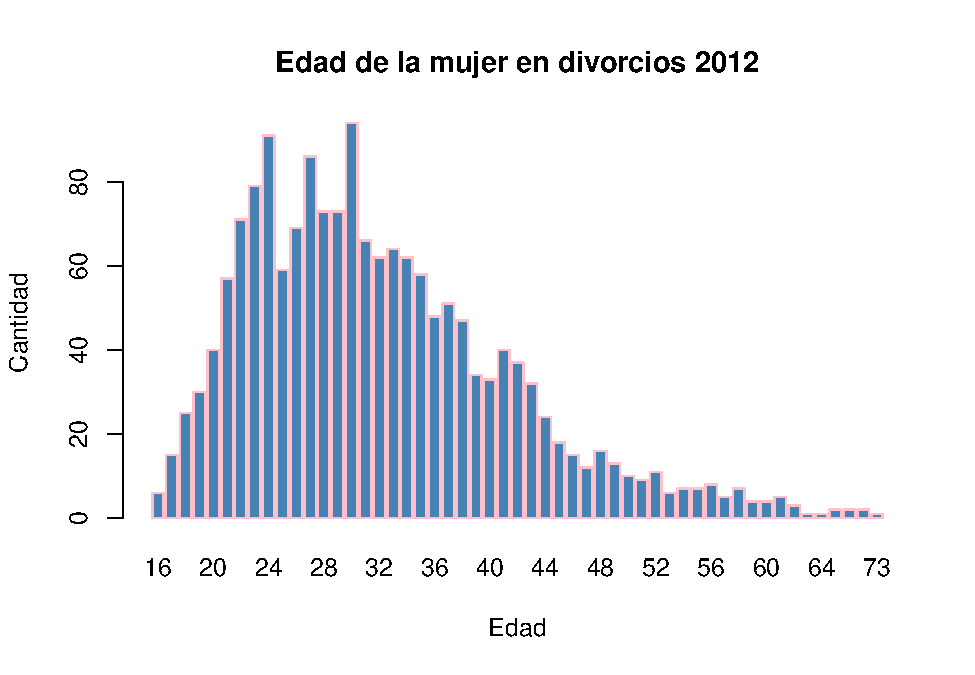
\includegraphics{Proyecto_files/figure-latex/unnamed-chunk-20-1.pdf}

2013

\begin{Shaded}
\begin{Highlighting}[]
\NormalTok{D2013 }\OtherTok{\textless{}{-}} \FunctionTok{subset}\NormalTok{(D2013, EDADMUJ }\SpecialCharTok{\textless{}} \DecValTok{999}\NormalTok{)}

\FunctionTok{barplot}\NormalTok{(}\FunctionTok{table}\NormalTok{(D2013}\SpecialCharTok{$}\NormalTok{EDADMUJ), }\AttributeTok{main =} \StringTok{"Edad de la mujer en divorcios 2013"}\NormalTok{, }\AttributeTok{xlab =} \StringTok{"Edad"}\NormalTok{, }\AttributeTok{ylab =} \StringTok{"Cantidad"}\NormalTok{, }\AttributeTok{col =} \StringTok{"steelblue"}\NormalTok{ , }\AttributeTok{border =} \StringTok{"pink"}\NormalTok{)}
\end{Highlighting}
\end{Shaded}

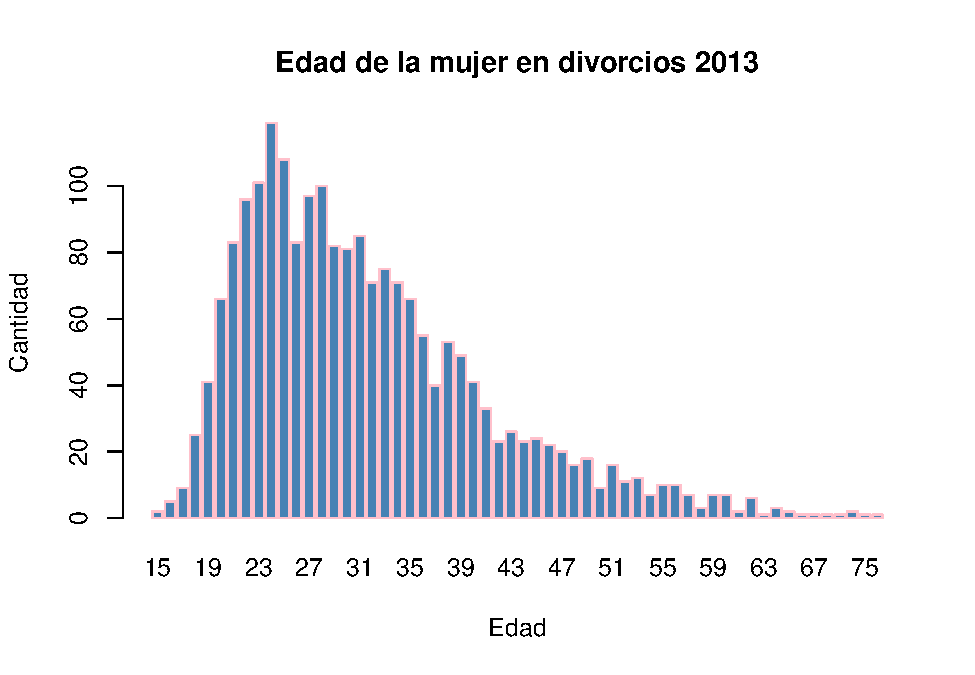
\includegraphics{Proyecto_files/figure-latex/unnamed-chunk-21-1.pdf}

2014

\begin{Shaded}
\begin{Highlighting}[]
\NormalTok{D2014 }\OtherTok{\textless{}{-}} \FunctionTok{subset}\NormalTok{(D2014, EDADMUJ }\SpecialCharTok{\textless{}} \DecValTok{999}\NormalTok{)}

\FunctionTok{barplot}\NormalTok{(}\FunctionTok{table}\NormalTok{(D2014}\SpecialCharTok{$}\NormalTok{EDADMUJ), }\AttributeTok{main =} \StringTok{"Edad de la mujer en divorcios 2014"}\NormalTok{, }\AttributeTok{xlab =} \StringTok{"Edad"}\NormalTok{, }\AttributeTok{ylab =} \StringTok{"Cantidad"}\NormalTok{, }\AttributeTok{col =} \StringTok{"steelblue"}\NormalTok{ , }\AttributeTok{border =} \StringTok{"pink"}\NormalTok{)}
\end{Highlighting}
\end{Shaded}

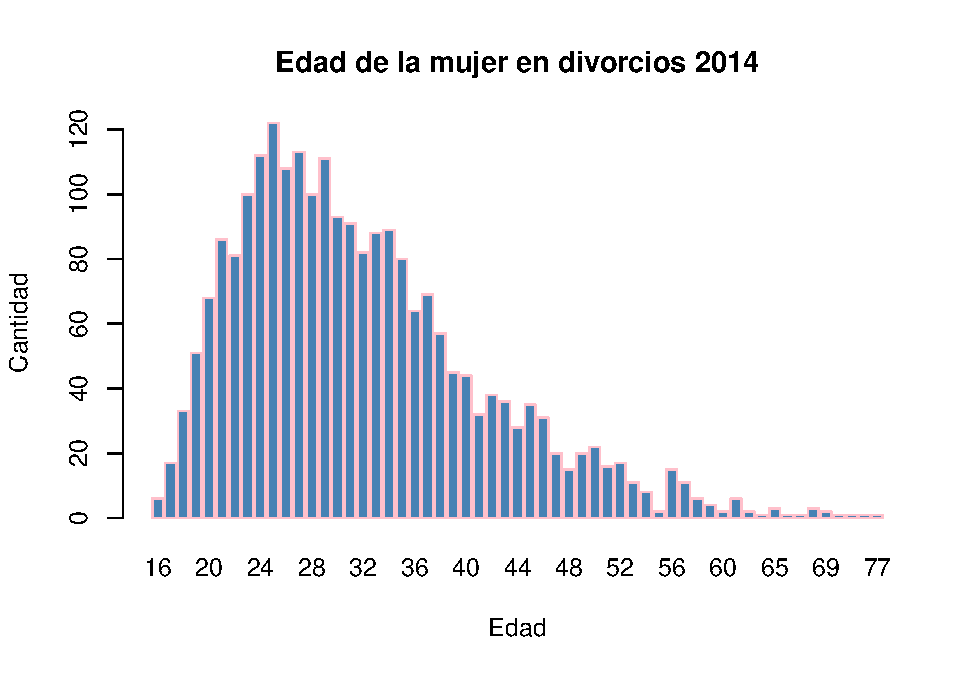
\includegraphics{Proyecto_files/figure-latex/unnamed-chunk-22-1.pdf}

2015

\begin{Shaded}
\begin{Highlighting}[]
\NormalTok{D2015 }\OtherTok{\textless{}{-}} \FunctionTok{subset}\NormalTok{(D2015, EDADMUJ }\SpecialCharTok{\textless{}} \DecValTok{999}\NormalTok{)}

\FunctionTok{barplot}\NormalTok{(}\FunctionTok{table}\NormalTok{(D2015}\SpecialCharTok{$}\NormalTok{EDADMUJ), }\AttributeTok{main =} \StringTok{"Edad de la mujer en divorcios 2015"}\NormalTok{, }\AttributeTok{xlab =} \StringTok{"Edad"}\NormalTok{, }\AttributeTok{ylab =} \StringTok{"Cantidad"}\NormalTok{, }\AttributeTok{col =} \StringTok{"steelblue"}\NormalTok{ , }\AttributeTok{border =} \StringTok{"pink"}\NormalTok{)}
\end{Highlighting}
\end{Shaded}

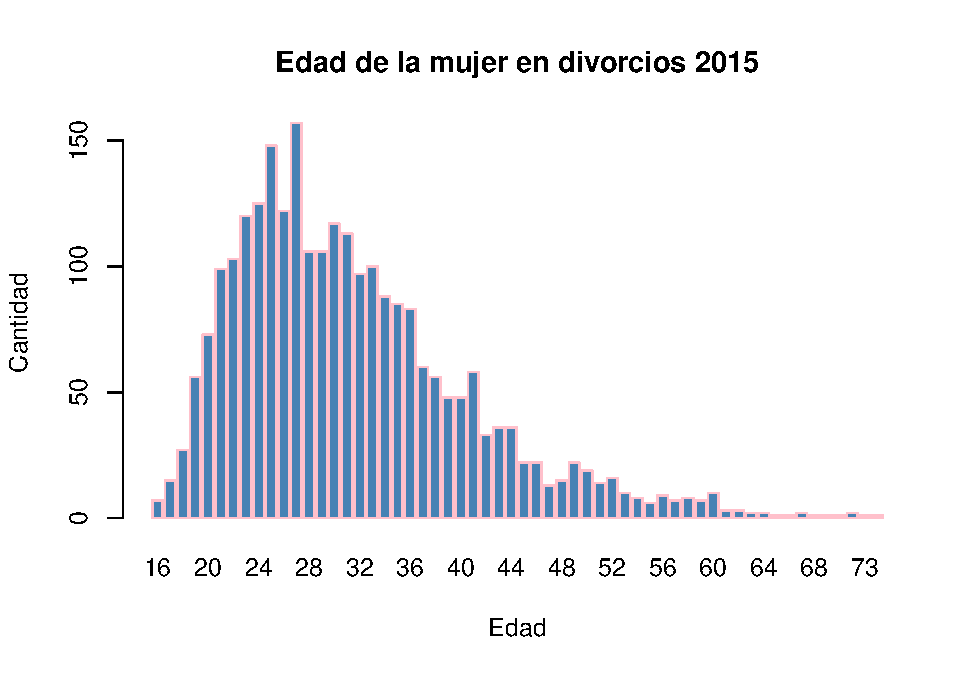
\includegraphics{Proyecto_files/figure-latex/unnamed-chunk-23-1.pdf}

2016

\begin{Shaded}
\begin{Highlighting}[]
\NormalTok{D2016 }\OtherTok{\textless{}{-}} \FunctionTok{subset}\NormalTok{(D2016, EDADMUJ }\SpecialCharTok{\textless{}} \DecValTok{999}\NormalTok{)}

\FunctionTok{barplot}\NormalTok{(}\FunctionTok{table}\NormalTok{(D2016}\SpecialCharTok{$}\NormalTok{EDADMUJ), }\AttributeTok{main =} \StringTok{"Edad de la mujer en divorcios 2016"}\NormalTok{, }\AttributeTok{xlab =} \StringTok{"Edad"}\NormalTok{, }\AttributeTok{ylab =} \StringTok{"Cantidad"}\NormalTok{, }\AttributeTok{col =} \StringTok{"steelblue"}\NormalTok{ , }\AttributeTok{border =} \StringTok{"pink"}\NormalTok{)}
\end{Highlighting}
\end{Shaded}

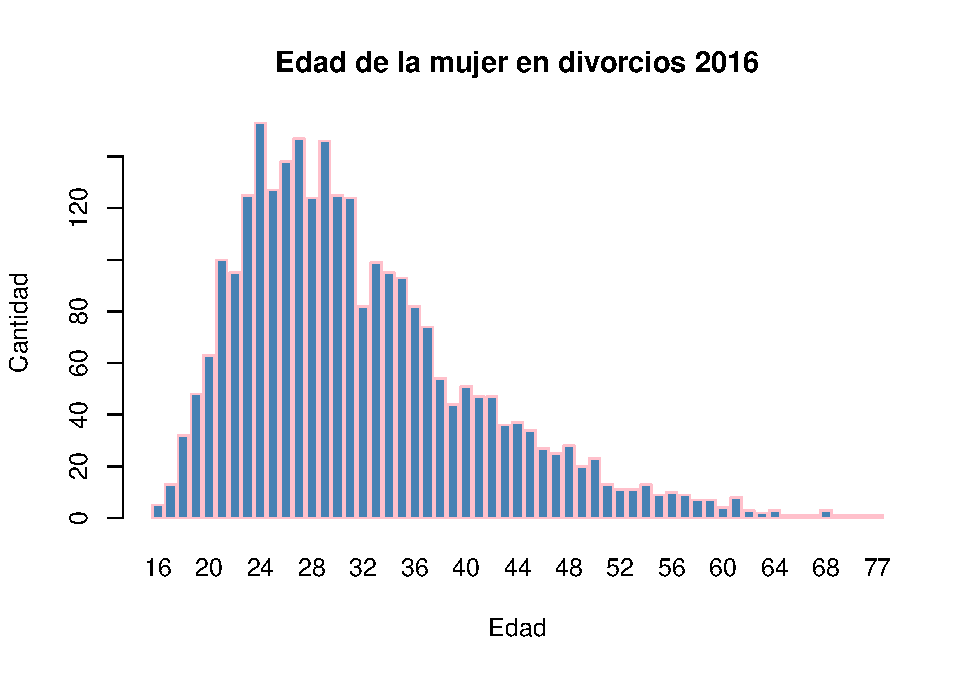
\includegraphics{Proyecto_files/figure-latex/unnamed-chunk-24-1.pdf}

2017

\begin{Shaded}
\begin{Highlighting}[]
\NormalTok{D2017 }\OtherTok{\textless{}{-}} \FunctionTok{subset}\NormalTok{(D2017, EDADMUJ }\SpecialCharTok{\textless{}} \DecValTok{999}\NormalTok{)}

\FunctionTok{barplot}\NormalTok{(}\FunctionTok{table}\NormalTok{(D2017}\SpecialCharTok{$}\NormalTok{EDADMUJ), }\AttributeTok{main =} \StringTok{"Edad de la mujer en divorcios 2017"}\NormalTok{, }\AttributeTok{xlab =} \StringTok{"Edad"}\NormalTok{, }\AttributeTok{ylab =} \StringTok{"Cantidad"}\NormalTok{, }\AttributeTok{col =} \StringTok{"steelblue"}\NormalTok{ , }\AttributeTok{border =} \StringTok{"pink"}\NormalTok{)}
\end{Highlighting}
\end{Shaded}

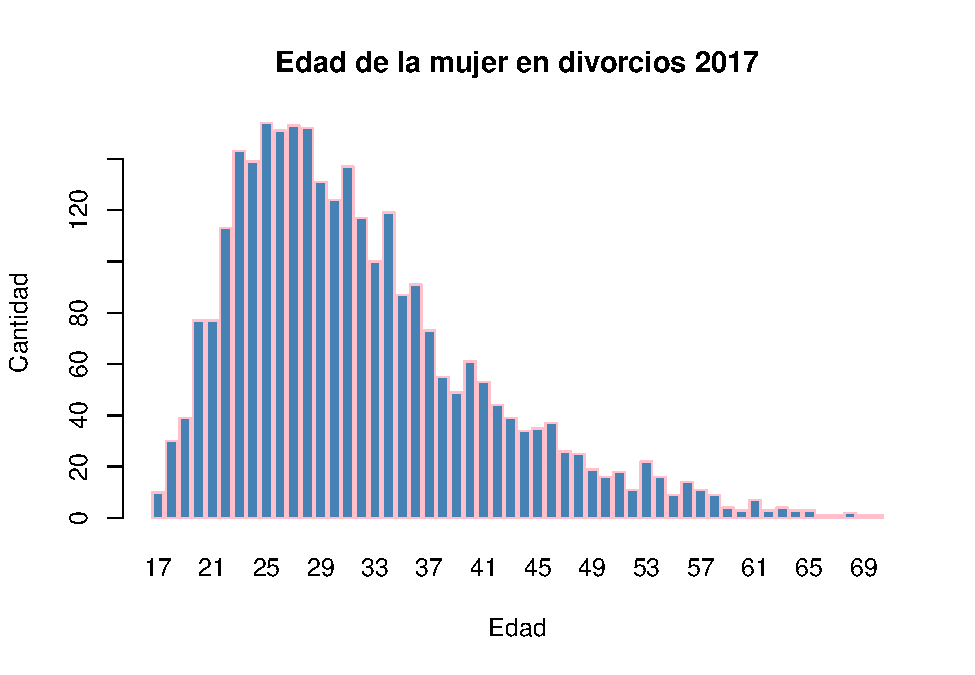
\includegraphics{Proyecto_files/figure-latex/unnamed-chunk-25-1.pdf}

2018

\begin{Shaded}
\begin{Highlighting}[]
\NormalTok{D2018 }\OtherTok{\textless{}{-}} \FunctionTok{subset}\NormalTok{(D2018, EDADMUJ }\SpecialCharTok{\textless{}} \DecValTok{999}\NormalTok{)}

\FunctionTok{barplot}\NormalTok{(}\FunctionTok{table}\NormalTok{(D2018}\SpecialCharTok{$}\NormalTok{EDADMUJ), }\AttributeTok{main =} \StringTok{"Edad de la mujer en divorcios 2018"}\NormalTok{, }\AttributeTok{xlab =} \StringTok{"Edad"}\NormalTok{, }\AttributeTok{ylab =} \StringTok{"Cantidad"}\NormalTok{, }\AttributeTok{col =} \StringTok{"steelblue"}\NormalTok{ , }\AttributeTok{border =} \StringTok{"pink"}\NormalTok{)}
\end{Highlighting}
\end{Shaded}

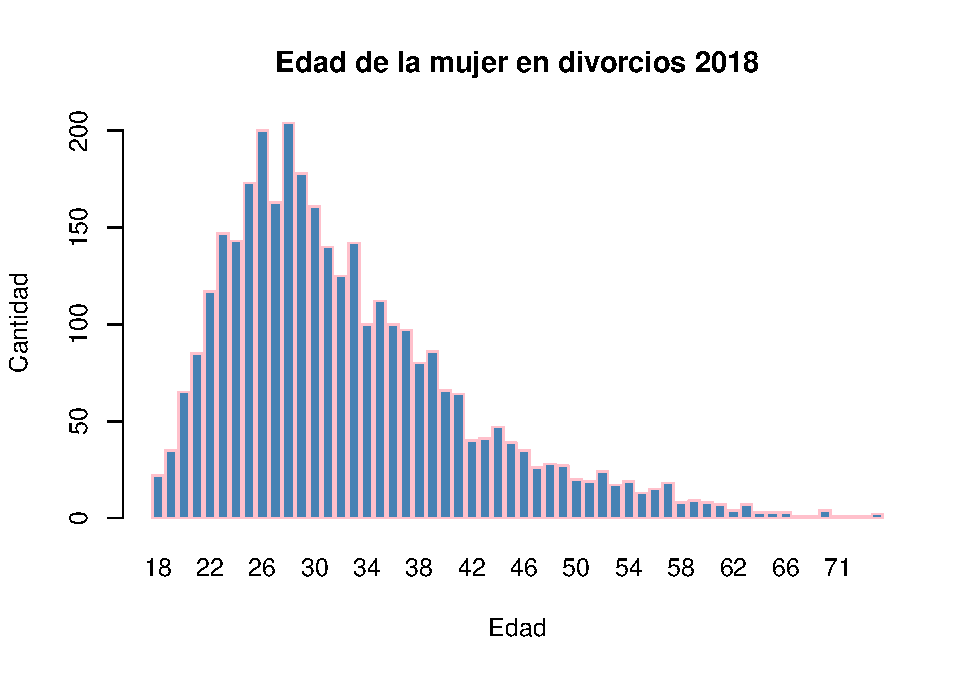
\includegraphics{Proyecto_files/figure-latex/unnamed-chunk-26-1.pdf}

2019

\begin{Shaded}
\begin{Highlighting}[]
\NormalTok{D2019 }\OtherTok{\textless{}{-}} \FunctionTok{subset}\NormalTok{(D2019, EDADMUJ }\SpecialCharTok{\textless{}} \DecValTok{999}\NormalTok{)}

\FunctionTok{barplot}\NormalTok{(}\FunctionTok{table}\NormalTok{(D2019}\SpecialCharTok{$}\NormalTok{EDADMUJ), }\AttributeTok{main =} \StringTok{"Edad de la mujer en divorcios 2019"}\NormalTok{, }\AttributeTok{xlab =} \StringTok{"Edad"}\NormalTok{, }\AttributeTok{ylab =} \StringTok{"Cantidad"}\NormalTok{, }\AttributeTok{col =} \StringTok{"steelblue"}\NormalTok{ , }\AttributeTok{border =} \StringTok{"pink"}\NormalTok{)}
\end{Highlighting}
\end{Shaded}

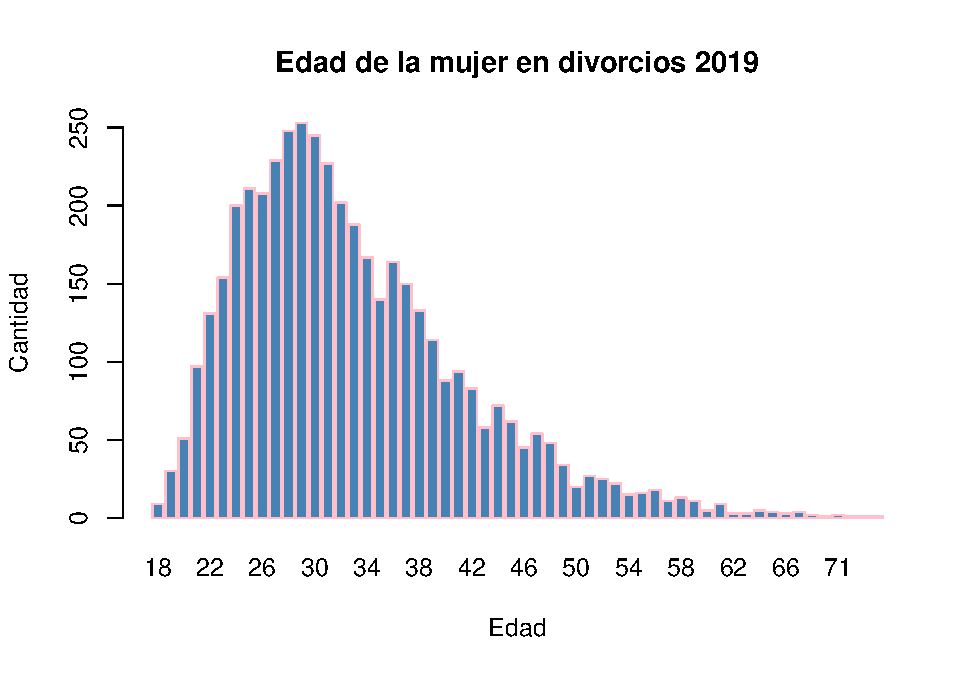
\includegraphics{Proyecto_files/figure-latex/unnamed-chunk-27-1.pdf}

2020

\begin{Shaded}
\begin{Highlighting}[]
\NormalTok{D2020 }\OtherTok{\textless{}{-}} \FunctionTok{subset}\NormalTok{(D2020, EDADMUJ }\SpecialCharTok{\textless{}} \DecValTok{999}\NormalTok{)}

\FunctionTok{barplot}\NormalTok{(}\FunctionTok{table}\NormalTok{(D2020}\SpecialCharTok{$}\NormalTok{EDADMUJ), }\AttributeTok{main =} \StringTok{"Edad de la mujer en divorcios 2020"}\NormalTok{, }\AttributeTok{xlab =} \StringTok{"Edad"}\NormalTok{, }\AttributeTok{ylab =} \StringTok{"Cantidad"}\NormalTok{, }\AttributeTok{col =} \StringTok{"steelblue"}\NormalTok{ , }\AttributeTok{border =} \StringTok{"pink"}\NormalTok{)}
\end{Highlighting}
\end{Shaded}

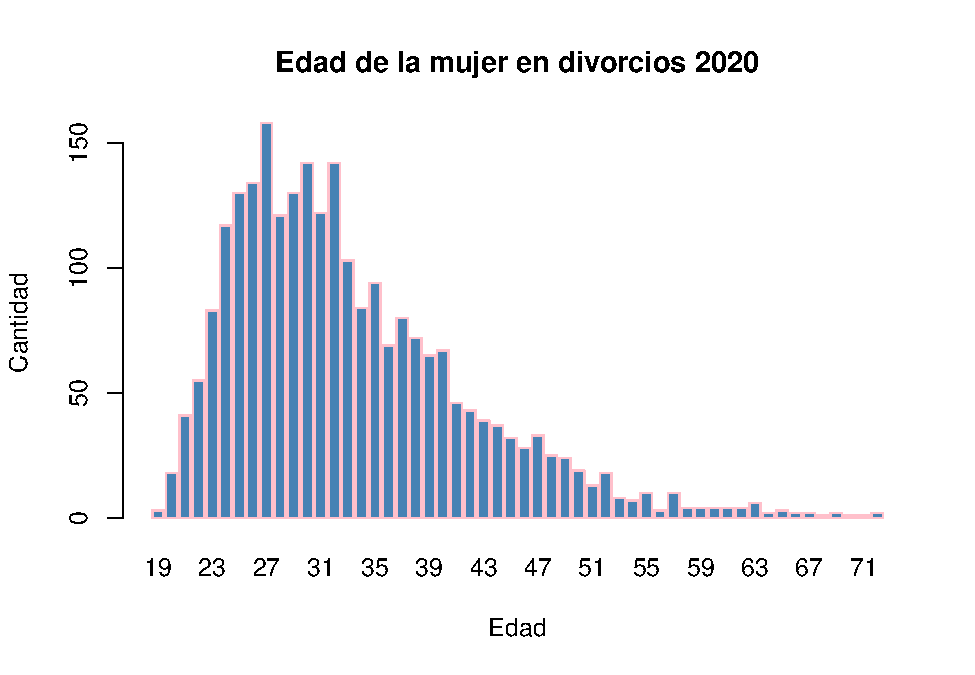
\includegraphics{Proyecto_files/figure-latex/unnamed-chunk-28-1.pdf}

2021

\begin{Shaded}
\begin{Highlighting}[]
\NormalTok{D2021 }\OtherTok{\textless{}{-}} \FunctionTok{subset}\NormalTok{(D2021, EDADMUJ }\SpecialCharTok{\textless{}} \DecValTok{999}\NormalTok{)}

\FunctionTok{barplot}\NormalTok{(}\FunctionTok{table}\NormalTok{(D2021}\SpecialCharTok{$}\NormalTok{EDADMUJ), }\AttributeTok{main =} \StringTok{"Edad de la mujer en divorcios 2021"}\NormalTok{, }\AttributeTok{xlab =} \StringTok{"Edad"}\NormalTok{, }\AttributeTok{ylab =} \StringTok{"Cantidad"}\NormalTok{, }\AttributeTok{col =} \StringTok{"steelblue"}\NormalTok{ , }\AttributeTok{border =} \StringTok{"pink"}\NormalTok{)}
\end{Highlighting}
\end{Shaded}

\hypertarget{section}{%
\subsection[]{\texorpdfstring{\protect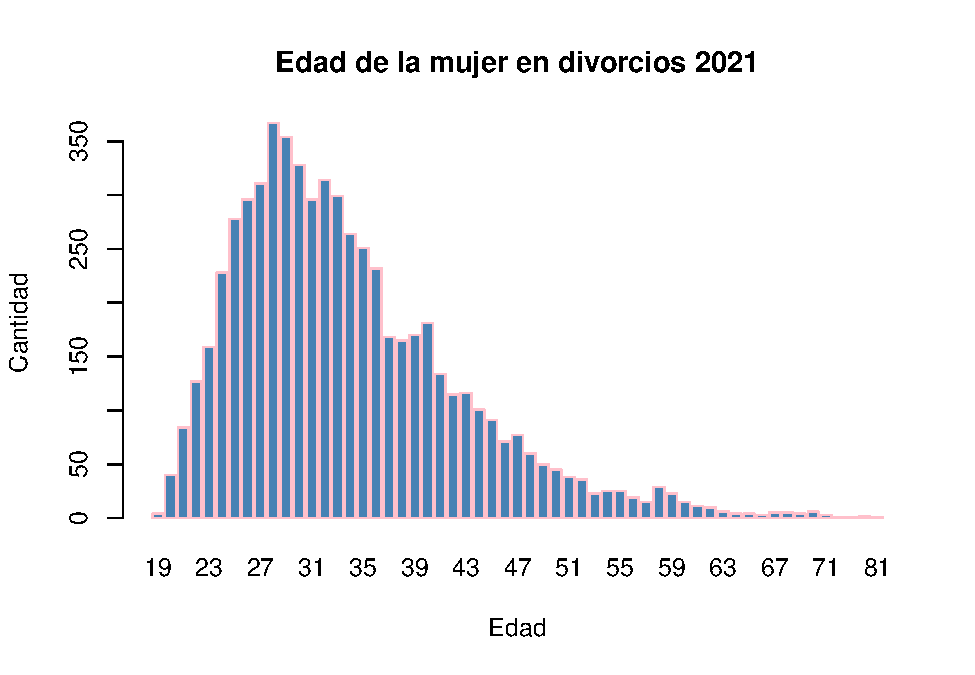
\includegraphics{Proyecto_files/figure-latex/unnamed-chunk-29-1.pdf}}{}}\label{section}}

\hypertarget{combinando-datos}{%
\subsection{Combinando datos}\label{combinando-datos}}

\begin{Shaded}
\begin{Highlighting}[]
\FunctionTok{colnames}\NormalTok{(D2009) }\OtherTok{\textless{}{-}} \FunctionTok{c}\NormalTok{(}\StringTok{"DEPREG"}\NormalTok{, }\StringTok{"MUPREG"}\NormalTok{, }\StringTok{"MESREG"}\NormalTok{, }\StringTok{"AÑOREG"}\NormalTok{, }\StringTok{"DIAOCU"}\NormalTok{, }\StringTok{"MESOCU"}\NormalTok{, }\StringTok{"AÑOOCU"}\NormalTok{, }\StringTok{"DEPOCU"}\NormalTok{, }\StringTok{"MUPOCU"}\NormalTok{, }\StringTok{"EDADHOM"}\NormalTok{, }\StringTok{"EDADMUJ"}\NormalTok{, }\StringTok{"PPERHOM"}\NormalTok{, }\StringTok{"PPERMUJ"}\NormalTok{, }\StringTok{"NACHOM"}\NormalTok{, }\StringTok{"NACMUJ"}\NormalTok{, }\StringTok{"CIUOHOM"}\NormalTok{, }\StringTok{"CIUOMUJ"}\NormalTok{, }\StringTok{"Mever"}\NormalTok{, }\StringTok{"Anover"}\NormalTok{)}
\FunctionTok{colnames}\NormalTok{(D2010) }\OtherTok{\textless{}{-}} \FunctionTok{c}\NormalTok{(}\StringTok{"DEPREG"}\NormalTok{, }\StringTok{"MUPREG"}\NormalTok{, }\StringTok{"MESREG"}\NormalTok{, }\StringTok{"AÑOREG"}\NormalTok{, }\StringTok{"DIAOCU"}\NormalTok{, }\StringTok{"MESOCU"}\NormalTok{, }\StringTok{"AÑOOCU"}\NormalTok{, }\StringTok{"DEPOCU"}\NormalTok{, }\StringTok{"MUPOCU"}\NormalTok{, }\StringTok{"EDADHOM"}\NormalTok{, }\StringTok{"EDADMUJ"}\NormalTok{, }\StringTok{"PPERHOM"}\NormalTok{, }\StringTok{"PPERMUJ"}\NormalTok{, }\StringTok{"NACHOM"}\NormalTok{, }\StringTok{"NACMUJ"}\NormalTok{, }\StringTok{"ESCHOM"}\NormalTok{, }\StringTok{"ESCMUJ"}\NormalTok{, }\StringTok{"CIUOHOM"}\NormalTok{, }\StringTok{"CIUOMUJ"}\NormalTok{)}
\FunctionTok{colnames}\NormalTok{(D2011) }\OtherTok{\textless{}{-}} \FunctionTok{c}\NormalTok{(}\StringTok{"DEPREG"}\NormalTok{, }\StringTok{"MUPREG"}\NormalTok{, }\StringTok{"MESREG"}\NormalTok{, }\StringTok{"AÑOREG"}\NormalTok{, }\StringTok{"DIAOCU"}\NormalTok{, }\StringTok{"MESOCU"}\NormalTok{, }\StringTok{"AÑOOCU"}\NormalTok{, }\StringTok{"DEPOCU"}\NormalTok{, }\StringTok{"MUPOCU"}\NormalTok{, }\StringTok{"EDADHOM"}\NormalTok{, }\StringTok{"EDADMUJ"}\NormalTok{, }\StringTok{"PPERHOM"}\NormalTok{, }\StringTok{"PPERMUJ"}\NormalTok{, }\StringTok{"NACHOM"}\NormalTok{, }\StringTok{"NACMUJ"}\NormalTok{, }\StringTok{"ESCHOM"}\NormalTok{, }\StringTok{"ESCMUJ"}\NormalTok{, }\StringTok{"CIUOHOM"}\NormalTok{, }\StringTok{"CIUOMUJ"}\NormalTok{)}
\FunctionTok{colnames}\NormalTok{(D2012) }\OtherTok{\textless{}{-}} \FunctionTok{c}\NormalTok{(}\StringTok{"DEPREG"}\NormalTok{,  }\StringTok{"MUPREG"}\NormalTok{,  }\StringTok{"MESREG"}\NormalTok{,  }\StringTok{"AÑOREG"}\NormalTok{,  }\StringTok{"DIAOCU"}\NormalTok{,  }\StringTok{"MESOCU"}\NormalTok{,  }\StringTok{"DEPOCU"}\NormalTok{,  }\StringTok{"MUPOCU"}\NormalTok{, }\StringTok{"EDADHOM"}\NormalTok{, }\StringTok{"EDADMUJ"}\NormalTok{, }\StringTok{"PPERHOM"}\NormalTok{,  }\StringTok{"PPERMUJ"}\NormalTok{,  }\StringTok{"NACHOM"}\NormalTok{,  }\StringTok{"NACMUJ"}\NormalTok{,  }\StringTok{"ESCHOM"}\NormalTok{,  }\StringTok{"ESCMUJ"}\NormalTok{, }\StringTok{"CIUOHOM"}\NormalTok{,  }\StringTok{"CIUOMUJ"}\NormalTok{) }
\FunctionTok{colnames}\NormalTok{(D2013) }\OtherTok{\textless{}{-}} \FunctionTok{c}\NormalTok{( }\StringTok{"DEPREG"}\NormalTok{,  }\StringTok{"MUPREG"}\NormalTok{,  }\StringTok{"MESREG"}\NormalTok{,  }\StringTok{"AÑOREG"}\NormalTok{,  }\StringTok{"DIAOCU"}\NormalTok{,  }\StringTok{"MESOCU"}\NormalTok{,  }\StringTok{"DEPOCU"}\NormalTok{,  }\StringTok{"MUPOCU"}\NormalTok{,  }\StringTok{"EDADHOM"}\NormalTok{, }\StringTok{"EDADMUJ"}\NormalTok{, }\StringTok{"PPERHOM"}\NormalTok{,  }\StringTok{"PPERMUJ"}\NormalTok{,  }\StringTok{"NACHOM"}\NormalTok{,  }\StringTok{"NACMUJ"}\NormalTok{,  }\StringTok{"ESCHOM"}\NormalTok{,  }\StringTok{"ESCMUJ"}\NormalTok{,  }\StringTok{"CIUOHOM"}\NormalTok{, }\StringTok{"CIUOMUJ"}\NormalTok{)}
\FunctionTok{colnames}\NormalTok{(D2014) }\OtherTok{\textless{}{-}} \FunctionTok{c}\NormalTok{( }\StringTok{"DEPREG"}\NormalTok{,  }\StringTok{"MUPREG"}\NormalTok{,  }\StringTok{"MESREG"}\NormalTok{,  }\StringTok{"AÑOREG"}\NormalTok{,  }\StringTok{"DIAOCU"}\NormalTok{,  }\StringTok{"MESOCU"}\NormalTok{,  }\StringTok{"DEPOCU"}\NormalTok{,  }\StringTok{"MUPOCU"}\NormalTok{, }\StringTok{"EDADHOM"}\NormalTok{, }\StringTok{"EDADMUJ"}\NormalTok{, }\StringTok{"PPERHOM"}\NormalTok{,  }\StringTok{"PPERMUJ"}\NormalTok{,  }\StringTok{"NACHOM"}\NormalTok{,  }\StringTok{"NACMUJ"}\NormalTok{,  }\StringTok{"ESCHOM"}\NormalTok{,  }\StringTok{"ESCMUJ"}\NormalTok{,  }\StringTok{"CIUOHOM"}\NormalTok{, }\StringTok{"CIUOMUJ"}\NormalTok{)}
\FunctionTok{colnames}\NormalTok{(D2015) }\OtherTok{\textless{}{-}} \FunctionTok{c}\NormalTok{(}\StringTok{"DEPREG"}\NormalTok{,  }\StringTok{"MUPREG"}\NormalTok{,  }\StringTok{"MESREG"}\NormalTok{,  }\StringTok{"AÑOREG"}\NormalTok{,  }\StringTok{"DIAOCU"}\NormalTok{,  }\StringTok{"MESOCU"}\NormalTok{,  }\StringTok{"AÑOOCU"}\NormalTok{,  }\StringTok{"DEPOCU"}\NormalTok{,  }\StringTok{"MUPOCU"}\NormalTok{,  }\StringTok{"EDADHOM"}\NormalTok{, }\StringTok{"EDADMUJ"}\NormalTok{, }\StringTok{"PPERHOM"}\NormalTok{, }\StringTok{"PPERMUJ"}\NormalTok{,  }\StringTok{"NACHOM"}\NormalTok{, }\StringTok{"NACMUJ"}\NormalTok{,  }\StringTok{"ESCHOM"}\NormalTok{,  }\StringTok{"ESCMUJ"}\NormalTok{,  }\StringTok{"CIUOHOM"}\NormalTok{, }\StringTok{"CIUOMUJ"}\NormalTok{)}
\end{Highlighting}
\end{Shaded}

\begin{Shaded}
\begin{Highlighting}[]
\NormalTok{D2009 }\OtherTok{\textless{}{-}}\NormalTok{ D2009 }\SpecialCharTok{\%\textgreater{}\%} \FunctionTok{mutate}\NormalTok{(AÑOREG }\OtherTok{=} \FunctionTok{as.numeric}\NormalTok{(AÑOREG))}
\NormalTok{D2010 }\OtherTok{\textless{}{-}}\NormalTok{ D2010 }\SpecialCharTok{\%\textgreater{}\%} \FunctionTok{mutate}\NormalTok{(AÑOREG }\OtherTok{=} \FunctionTok{as.numeric}\NormalTok{(AÑOREG))}
\NormalTok{D2011 }\OtherTok{\textless{}{-}}\NormalTok{ D2011 }\SpecialCharTok{\%\textgreater{}\%} \FunctionTok{mutate}\NormalTok{(AÑOREG }\OtherTok{=} \FunctionTok{as.numeric}\NormalTok{(AÑOREG))}
\NormalTok{D2012 }\OtherTok{\textless{}{-}}\NormalTok{ D2012 }\SpecialCharTok{\%\textgreater{}\%} \FunctionTok{mutate}\NormalTok{(AÑOREG }\OtherTok{=} \FunctionTok{as.numeric}\NormalTok{(AÑOREG))}
\NormalTok{D2013 }\OtherTok{\textless{}{-}}\NormalTok{ D2013 }\SpecialCharTok{\%\textgreater{}\%} \FunctionTok{mutate}\NormalTok{(AÑOREG }\OtherTok{=} \FunctionTok{as.numeric}\NormalTok{(AÑOREG))}
\NormalTok{D2014 }\OtherTok{\textless{}{-}}\NormalTok{ D2014 }\SpecialCharTok{\%\textgreater{}\%} \FunctionTok{mutate}\NormalTok{(AÑOREG }\OtherTok{=} \FunctionTok{as.numeric}\NormalTok{(AÑOREG))}
\NormalTok{D2015 }\OtherTok{\textless{}{-}}\NormalTok{ D2015 }\SpecialCharTok{\%\textgreater{}\%} \FunctionTok{mutate}\NormalTok{(AÑOREG }\OtherTok{=} \FunctionTok{as.numeric}\NormalTok{(AÑOREG))}
\NormalTok{D2016 }\OtherTok{\textless{}{-}}\NormalTok{ D2016 }\SpecialCharTok{\%\textgreater{}\%} \FunctionTok{mutate}\NormalTok{(AÑOREG }\OtherTok{=} \FunctionTok{as.numeric}\NormalTok{(AÑOREG))}
\NormalTok{D2017 }\OtherTok{\textless{}{-}}\NormalTok{ D2017 }\SpecialCharTok{\%\textgreater{}\%} \FunctionTok{mutate}\NormalTok{(AÑOREG }\OtherTok{=} \FunctionTok{as.numeric}\NormalTok{(AÑOREG))}
\NormalTok{D2018 }\OtherTok{\textless{}{-}}\NormalTok{ D2018 }\SpecialCharTok{\%\textgreater{}\%} \FunctionTok{mutate}\NormalTok{(AÑOREG }\OtherTok{=} \FunctionTok{as.numeric}\NormalTok{(AÑOREG))}
\NormalTok{D2019 }\OtherTok{\textless{}{-}}\NormalTok{ D2019 }\SpecialCharTok{\%\textgreater{}\%} \FunctionTok{mutate}\NormalTok{(AÑOREG }\OtherTok{=} \FunctionTok{as.numeric}\NormalTok{(AÑOREG))}
\NormalTok{D2020 }\OtherTok{\textless{}{-}}\NormalTok{ D2020 }\SpecialCharTok{\%\textgreater{}\%} \FunctionTok{mutate}\NormalTok{(AÑOREG }\OtherTok{=} \FunctionTok{as.numeric}\NormalTok{(AÑOREG))}
\NormalTok{D2021 }\OtherTok{\textless{}{-}}\NormalTok{ D2021 }\SpecialCharTok{\%\textgreater{}\%} \FunctionTok{mutate}\NormalTok{(AÑOREG }\OtherTok{=} \FunctionTok{as.numeric}\NormalTok{(AÑOREG))}
\end{Highlighting}
\end{Shaded}

\begin{Shaded}
\begin{Highlighting}[]
\NormalTok{D2009 }\OtherTok{\textless{}{-}}\NormalTok{ D2009 }\SpecialCharTok{\%\textgreater{}\%} \FunctionTok{mutate}\NormalTok{(AÑOOCU }\OtherTok{=} \FunctionTok{as.numeric}\NormalTok{(AÑOOCU))}
\NormalTok{D2010 }\OtherTok{\textless{}{-}}\NormalTok{ D2010 }\SpecialCharTok{\%\textgreater{}\%} \FunctionTok{mutate}\NormalTok{(AÑOOCU }\OtherTok{=} \FunctionTok{as.numeric}\NormalTok{(AÑOOCU))}
\NormalTok{D2011 }\OtherTok{\textless{}{-}}\NormalTok{ D2011 }\SpecialCharTok{\%\textgreater{}\%} \FunctionTok{mutate}\NormalTok{(AÑOOCU }\OtherTok{=} \FunctionTok{as.numeric}\NormalTok{(AÑOOCU))}
\end{Highlighting}
\end{Shaded}

\begin{Shaded}
\begin{Highlighting}[]
\NormalTok{D2009 }\OtherTok{\textless{}{-}}\NormalTok{ D2009 }\SpecialCharTok{\%\textgreater{}\%} \FunctionTok{mutate}\NormalTok{(}\AttributeTok{CIUOHOM =} \FunctionTok{as.character}\NormalTok{(CIUOHOM))}
\NormalTok{D2010 }\OtherTok{\textless{}{-}}\NormalTok{ D2010 }\SpecialCharTok{\%\textgreater{}\%} \FunctionTok{mutate}\NormalTok{(}\AttributeTok{CIUOHOM =} \FunctionTok{as.character}\NormalTok{(CIUOHOM))}
\NormalTok{D2011 }\OtherTok{\textless{}{-}}\NormalTok{ D2011 }\SpecialCharTok{\%\textgreater{}\%} \FunctionTok{mutate}\NormalTok{(}\AttributeTok{CIUOHOM =} \FunctionTok{as.character}\NormalTok{(CIUOHOM))}
\NormalTok{D2012 }\OtherTok{\textless{}{-}}\NormalTok{ D2012 }\SpecialCharTok{\%\textgreater{}\%} \FunctionTok{mutate}\NormalTok{(}\AttributeTok{CIUOHOM =} \FunctionTok{as.character}\NormalTok{(CIUOHOM))}
\NormalTok{D2013 }\OtherTok{\textless{}{-}}\NormalTok{ D2013 }\SpecialCharTok{\%\textgreater{}\%} \FunctionTok{mutate}\NormalTok{(}\AttributeTok{CIUOHOM =} \FunctionTok{as.character}\NormalTok{(CIUOHOM))}
\NormalTok{D2014 }\OtherTok{\textless{}{-}}\NormalTok{ D2014 }\SpecialCharTok{\%\textgreater{}\%} \FunctionTok{mutate}\NormalTok{(}\AttributeTok{CIUOHOM =} \FunctionTok{as.character}\NormalTok{(CIUOHOM))}
\NormalTok{D2015 }\OtherTok{\textless{}{-}}\NormalTok{ D2015 }\SpecialCharTok{\%\textgreater{}\%} \FunctionTok{mutate}\NormalTok{(}\AttributeTok{CIUOHOM =} \FunctionTok{as.character}\NormalTok{(CIUOHOM))}
\NormalTok{D2016 }\OtherTok{\textless{}{-}}\NormalTok{ D2016 }\SpecialCharTok{\%\textgreater{}\%} \FunctionTok{mutate}\NormalTok{(}\AttributeTok{CIUOHOM =} \FunctionTok{as.character}\NormalTok{(CIUOHOM))}
\NormalTok{D2017 }\OtherTok{\textless{}{-}}\NormalTok{ D2017 }\SpecialCharTok{\%\textgreater{}\%} \FunctionTok{mutate}\NormalTok{(}\AttributeTok{CIUOHOM =} \FunctionTok{as.character}\NormalTok{(CIUOHOM))}
\NormalTok{D2018 }\OtherTok{\textless{}{-}}\NormalTok{ D2018 }\SpecialCharTok{\%\textgreater{}\%} \FunctionTok{mutate}\NormalTok{(}\AttributeTok{CIUOHOM =} \FunctionTok{as.character}\NormalTok{(CIUOHOM))}
\NormalTok{D2019 }\OtherTok{\textless{}{-}}\NormalTok{ D2019 }\SpecialCharTok{\%\textgreater{}\%} \FunctionTok{mutate}\NormalTok{(}\AttributeTok{CIUOHOM =} \FunctionTok{as.character}\NormalTok{(CIUOHOM))}
\NormalTok{D2020 }\OtherTok{\textless{}{-}}\NormalTok{ D2020 }\SpecialCharTok{\%\textgreater{}\%} \FunctionTok{mutate}\NormalTok{(}\AttributeTok{CIUOHOM =} \FunctionTok{as.character}\NormalTok{(CIUOHOM))}
\NormalTok{D2021 }\OtherTok{\textless{}{-}}\NormalTok{ D2021 }\SpecialCharTok{\%\textgreater{}\%} \FunctionTok{mutate}\NormalTok{(}\AttributeTok{CIUOHOM =} \FunctionTok{as.character}\NormalTok{(CIUOHOM))}
\end{Highlighting}
\end{Shaded}

\begin{Shaded}
\begin{Highlighting}[]
\NormalTok{D2009 }\OtherTok{\textless{}{-}}\NormalTok{ D2009 }\SpecialCharTok{\%\textgreater{}\%} \FunctionTok{mutate}\NormalTok{(}\AttributeTok{CIUOMUJ =} \FunctionTok{as.character}\NormalTok{(CIUOMUJ))}
\NormalTok{D2010 }\OtherTok{\textless{}{-}}\NormalTok{ D2010 }\SpecialCharTok{\%\textgreater{}\%} \FunctionTok{mutate}\NormalTok{(}\AttributeTok{CIUOMUJ =} \FunctionTok{as.character}\NormalTok{(CIUOMUJ))}
\NormalTok{D2011 }\OtherTok{\textless{}{-}}\NormalTok{ D2011 }\SpecialCharTok{\%\textgreater{}\%} \FunctionTok{mutate}\NormalTok{(}\AttributeTok{CIUOMUJ =} \FunctionTok{as.character}\NormalTok{(CIUOMUJ))}
\NormalTok{D2012 }\OtherTok{\textless{}{-}}\NormalTok{ D2012 }\SpecialCharTok{\%\textgreater{}\%} \FunctionTok{mutate}\NormalTok{(}\AttributeTok{CIUOMUJ =} \FunctionTok{as.character}\NormalTok{(CIUOMUJ))}
\NormalTok{D2013 }\OtherTok{\textless{}{-}}\NormalTok{ D2013 }\SpecialCharTok{\%\textgreater{}\%} \FunctionTok{mutate}\NormalTok{(}\AttributeTok{CIUOMUJ =} \FunctionTok{as.character}\NormalTok{(CIUOMUJ))}
\NormalTok{D2014 }\OtherTok{\textless{}{-}}\NormalTok{ D2014 }\SpecialCharTok{\%\textgreater{}\%} \FunctionTok{mutate}\NormalTok{(}\AttributeTok{CIUOMUJ =} \FunctionTok{as.character}\NormalTok{(CIUOMUJ))}
\NormalTok{D2015 }\OtherTok{\textless{}{-}}\NormalTok{ D2015 }\SpecialCharTok{\%\textgreater{}\%} \FunctionTok{mutate}\NormalTok{(}\AttributeTok{CIUOMUJ =} \FunctionTok{as.character}\NormalTok{(CIUOMUJ))}
\NormalTok{D2016 }\OtherTok{\textless{}{-}}\NormalTok{ D2016 }\SpecialCharTok{\%\textgreater{}\%} \FunctionTok{mutate}\NormalTok{(}\AttributeTok{CIUOMUJ =} \FunctionTok{as.character}\NormalTok{(CIUOMUJ))}
\NormalTok{D2017 }\OtherTok{\textless{}{-}}\NormalTok{ D2017 }\SpecialCharTok{\%\textgreater{}\%} \FunctionTok{mutate}\NormalTok{(}\AttributeTok{CIUOMUJ =} \FunctionTok{as.character}\NormalTok{(CIUOMUJ))}
\NormalTok{D2018 }\OtherTok{\textless{}{-}}\NormalTok{ D2018 }\SpecialCharTok{\%\textgreater{}\%} \FunctionTok{mutate}\NormalTok{(}\AttributeTok{CIUOMUJ =} \FunctionTok{as.character}\NormalTok{(CIUOMUJ))}
\NormalTok{D2019 }\OtherTok{\textless{}{-}}\NormalTok{ D2019 }\SpecialCharTok{\%\textgreater{}\%} \FunctionTok{mutate}\NormalTok{(}\AttributeTok{CIUOMUJ =} \FunctionTok{as.character}\NormalTok{(CIUOMUJ))}
\NormalTok{D2020 }\OtherTok{\textless{}{-}}\NormalTok{ D2020 }\SpecialCharTok{\%\textgreater{}\%} \FunctionTok{mutate}\NormalTok{(}\AttributeTok{CIUOMUJ =} \FunctionTok{as.character}\NormalTok{(CIUOMUJ))}
\NormalTok{D2021 }\OtherTok{\textless{}{-}}\NormalTok{ D2021 }\SpecialCharTok{\%\textgreater{}\%} \FunctionTok{mutate}\NormalTok{(}\AttributeTok{CIUOMUJ =} \FunctionTok{as.character}\NormalTok{(CIUOMUJ))}
\end{Highlighting}
\end{Shaded}

\begin{Shaded}
\begin{Highlighting}[]
\CommentTok{\#divorcios \textless{}{-} bind\_rows(D2009, D2010, D2011, D2012, D2013, D2014, D2015, D2016, D2017, D2018, D2019, D2020, D2021)}
\NormalTok{divorcios }\OtherTok{\textless{}{-}} \FunctionTok{bind\_rows}\NormalTok{( D2012, D2013, D2014, D2015, D2016, D2017, D2018, D2019, D2020, D2021)}
\CommentTok{\#l = list(D2012, D2013, D2014, D2015, D2016, D2017, D2018, D2019, D2020, D2021)}
\CommentTok{\#divorcios \textless{}{-} do.call("rbind",l)}
\end{Highlighting}
\end{Shaded}

\begin{Shaded}
\begin{Highlighting}[]
\FunctionTok{str}\NormalTok{(divorcios)}
\end{Highlighting}
\end{Shaded}

\begin{verbatim}
## tibble [30,378 x 19] (S3: tbl_df/tbl/data.frame)
##  $ DEPREG : dbl+lbl [1:30378] 17, 12,  1, 14,  1,  1,  1,  1,  1,  1,  9, 22,  3, ...
##    ..@ labels: Named num [1:22] 1 2 3 4 5 6 7 8 9 10 ...
##    .. ..- attr(*, "names")= chr [1:22] "Guatemala" "El Progreso" "Sacatepequez" "Chimaltenango" ...
##    ..@ label : chr "Departamento de registro"
##  $ MUPREG : chr+lbl [1:30378] 1708, 1213, 0101, 1416, 0101, 0101, 0101, 0101, 0101...
##    ..@ labels: Named chr [1:342] "1010" "2010" "0110" "1210" ...
##    .. ..- attr(*, "names")= chr [1:342] "San Antonio Suchitepéquez" "San Jacinto" "San Juan Sacatepéquez" "Tejutla" ...
##    ..@ label : chr "Municipio de registro"
##  $ MESREG : dbl+lbl [1:30378]  3,  5,  4,  6, 10,  2,  8, 11,  9,  8,  4,  1,  4, ...
##    ..@ labels: Named num [1:12] 1 2 3 4 5 6 7 8 9 10 ...
##    .. ..- attr(*, "names")= chr [1:12] "Enero" "Febrero" "Marzo" "Abril" ...
##    ..@ label : chr "Mes de registro"
##  $ AÑOREG : num [1:30378] 2012 2012 2012 2012 2012 ...
##  $ DIAOCU : num [1:30378] 16 3 27 28 12 9 11 3 29 16 ...
##  $ MESOCU : dbl+lbl [1:30378]  2,  2,  3,  5,  3,  1,  6,  8,  2,  5,  5,  2,  4, ...
##    ..@ label      : chr "Mes de ocurrencia"
##    ..@ format.spss: chr "F2.0"
##    ..@ labels     : Named num [1:12] 1 2 3 4 5 6 7 8 9 10 ...
##    .. ..- attr(*, "names")= chr [1:12] "Enero" "Febrero" "Marzo" "Abril" ...
##  $ DEPOCU : dbl+lbl [1:30378] 17, 12,  1, 14,  1,  1,  1,  1,  1,  1,  9, 22,  1, ...
##    ..@ labels: Named num [1:22] 1 2 3 4 5 6 7 8 9 10 ...
##    .. ..- attr(*, "names")= chr [1:22] "Guatemala" "El Progreso" "Sacatepequez" "Chimaltenango" ...
##    ..@ label : chr "Departamento de ocurrencia"
##  $ MUPOCU : chr+lbl [1:30378] 1703, 1215, 0101, 1401, 0101, 0101, 0101, 0101, 0101...
##    ..@ labels: Named chr [1:342] "1010" "2010" "0110" "1210" ...
##    .. ..- attr(*, "names")= chr [1:342] "San Antonio Suchitepéquez" "San Jacinto" "San Juan Sacatepéquez" "Tejutla" ...
##    ..@ label : chr "Municipio de ocurrencia"
##  $ EDADHOM: dbl+lbl [1:30378] 999,  35,  33,  31,  27,  37,  41,  36,  46,  38,  3...
##    ..@ label      : chr "Edad del hombre"
##    ..@ format.spss: chr "F4.0"
##    ..@ labels     : Named num 999
##    .. ..- attr(*, "names")= chr "Ignorado"
##  $ EDADMUJ: dbl+lbl [1:30378] 33, 30, 32, 28, 29, 30, 42, 30, 37, 35, 35, 33, 38, ...
##    ..@ label      : chr "Edad de la mujer"
##    ..@ format.spss: chr "F4.0"
##    ..@ labels     : Named num 999
##    .. ..- attr(*, "names")= chr "Ignorado"
##  $ PPERHOM: dbl+lbl [1:30378] 9, 2, 9, 9, 2, 9, 2, 2, 2, 2, 1, 9, 2, 2, 1, 2, 2, 9...
##    ..@ labels: Named num [1:6] 1 2 9 3 4 5
##    .. ..- attr(*, "names")= chr [1:6] "Indigena" "No indigena" "Ignorado" "Xinca" ...
##    ..@ label : chr "Grupo Etnico del hombre"
##  $ PPERMUJ: dbl+lbl [1:30378] 2, 2, 2, 2, 2, 9, 9, 2, 2, 2, 2, 2, 2, 2, 2, 2, 2, 9...
##    ..@ labels: Named num [1:6] 1 2 9 3 4 5
##    .. ..- attr(*, "names")= chr [1:6] "Indigena" "No indigena" "Ignorado" "Xinca" ...
##    ..@ label : chr "Grupo Etnico de la mujer"
##  $ NACHOM : dbl+lbl [1:30378] 320, 320, 320, 320, 320, 320, 320, 320, 320, 320, 32...
##    ..@ labels: Named num [1:105] 32 56 68 84 124 156 170 188 192 222 ...
##    .. ..- attr(*, "names")= chr [1:105] "Argentina" "Bélgica" "Bolivia" "Belice" ...
##    ..@ label : chr "Nacionalidad del hombre"
##  $ NACMUJ : dbl+lbl [1:30378] 320, 320, 320, 320, 320, 320, 320, 320, 320, 320, 32...
##    ..@ labels: Named num [1:103] 76 84 170 188 192 218 222 276 320 340 ...
##    .. ..- attr(*, "names")= chr [1:103] "Brasil" "Belice" "Colombia" "Costa Rica" ...
##    ..@ label : chr "Nacionalidad de la mujer"
##  $ ESCHOM : dbl+lbl [1:30378] 9, 5, 5, 1, 4, 9, 5, 5, 5, 9, 4, 9, 3, 5, 9, 9, 3, 9...
##    ..@ labels: Named num [1:8] 1 2 3 4 5 9 6 0
##    .. ..- attr(*, "names")= chr [1:8] "Ninguna" "Primaria" "Básico" "Diversificado" ...
##    ..@ label : chr "Escolaridad del hombre"
##  $ ESCMUJ : dbl+lbl [1:30378] 4, 9, 5, 4, 5, 9, 5, 5, 5, 5, 4, 4, 4, 5, 4, 5, 5, 9...
##    ..@ labels: Named num [1:8] 1 2 3 4 5 9 6 0
##    .. ..- attr(*, "names")= chr [1:8] "Ninguna" "Primaria" "Básico" "Diversificado" ...
##    ..@ label : chr "Escolaridad de la mujer"
##  $ CIUOHOM: chr [1:30378] "9712" "110" "2142" "8189" ...
##  $ CIUOMUJ: chr [1:30378] "110" "1120" "1120" "1120" ...
##  $ AÑOOCU : num [1:30378] NA NA NA NA NA NA NA NA NA NA ...
\end{verbatim}

\begin{verbatim}
## Warning: The dot-dot notation (`..density..`) was deprecated in ggplot2 3.4.0.
## i Please use `after_stat(density)` instead.
\end{verbatim}

\begin{verbatim}
## `stat_bin()` using `bins = 30`. Pick better value with `binwidth`.
\end{verbatim}

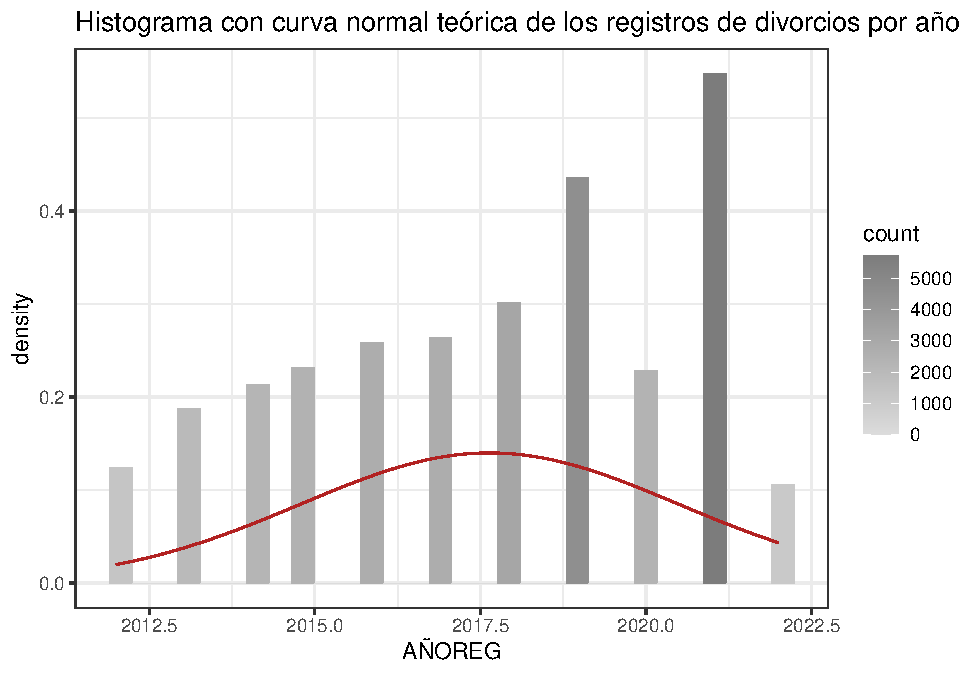
\includegraphics{Proyecto_files/figure-latex/normalHist-1.pdf}

\begin{Shaded}
\begin{Highlighting}[]
\FunctionTok{boxplot}\NormalTok{(divorcios}\SpecialCharTok{$}\NormalTok{AÑOREG, }\AttributeTok{main =} \StringTok{"Caja y Bigotes de registro de divorcios por año (2012 {-} 2021)"}\NormalTok{, }\AttributeTok{xlab =} \StringTok{"Registro por año"}\NormalTok{)}
\end{Highlighting}
\end{Shaded}

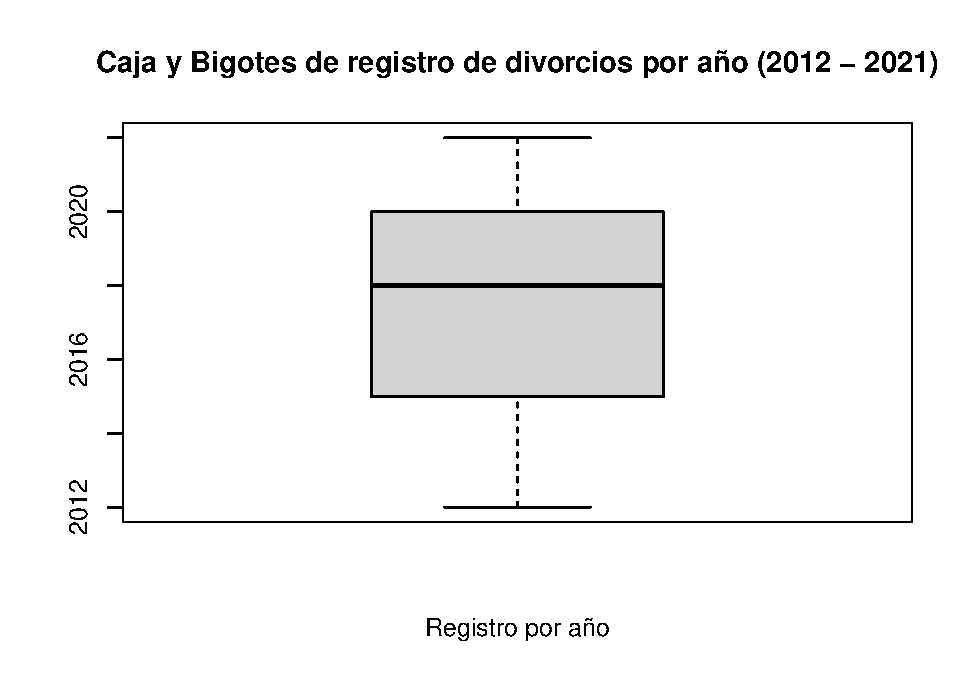
\includegraphics{Proyecto_files/figure-latex/unnamed-chunk-37-1.pdf}

\hypertarget{diagrama-de-qqnormal}{%
\subsubsection{Diagrama de qqnormal}\label{diagrama-de-qqnormal}}

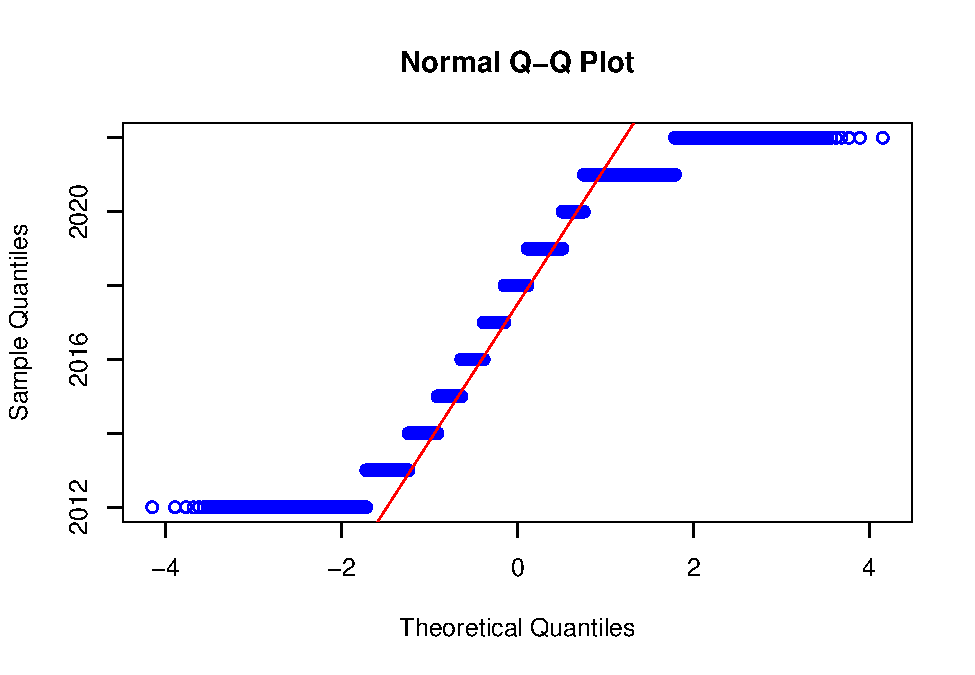
\includegraphics{Proyecto_files/figure-latex/normalQQ-1.pdf}

\hypertarget{registros-de-edad-hombre}{%
\subsection{Registros de Edad hombre}\label{registros-de-edad-hombre}}

\hypertarget{prueba-de-normalidad-para-la-edad-del-hombre}{%
\subsubsection{Prueba de normalidad para la edad del
hombre:}\label{prueba-de-normalidad-para-la-edad-del-hombre}}

\begin{verbatim}
## Don't know how to automatically pick scale for object of type
## <haven_labelled/vctrs_vctr/double>. Defaulting to continuous.
## `stat_bin()` using `bins = 30`. Pick better value with `binwidth`.
\end{verbatim}

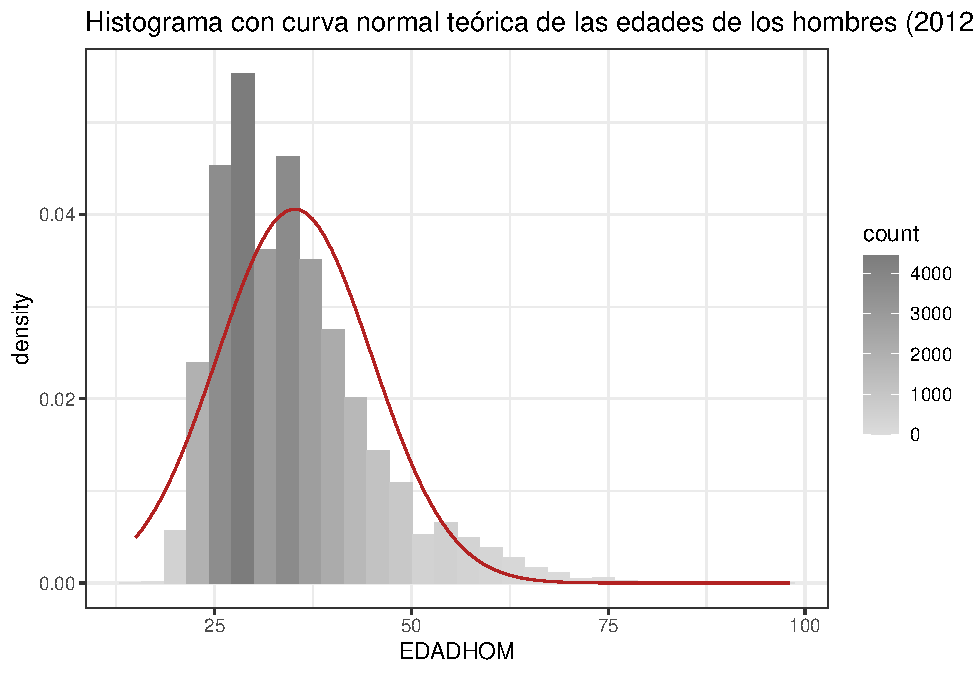
\includegraphics{Proyecto_files/figure-latex/normalHistEdadHombre-1.pdf}

\hypertarget{diagrama-de-caja-y-bigotes}{%
\subsubsection{Diagrama de caja y
bigotes}\label{diagrama-de-caja-y-bigotes}}

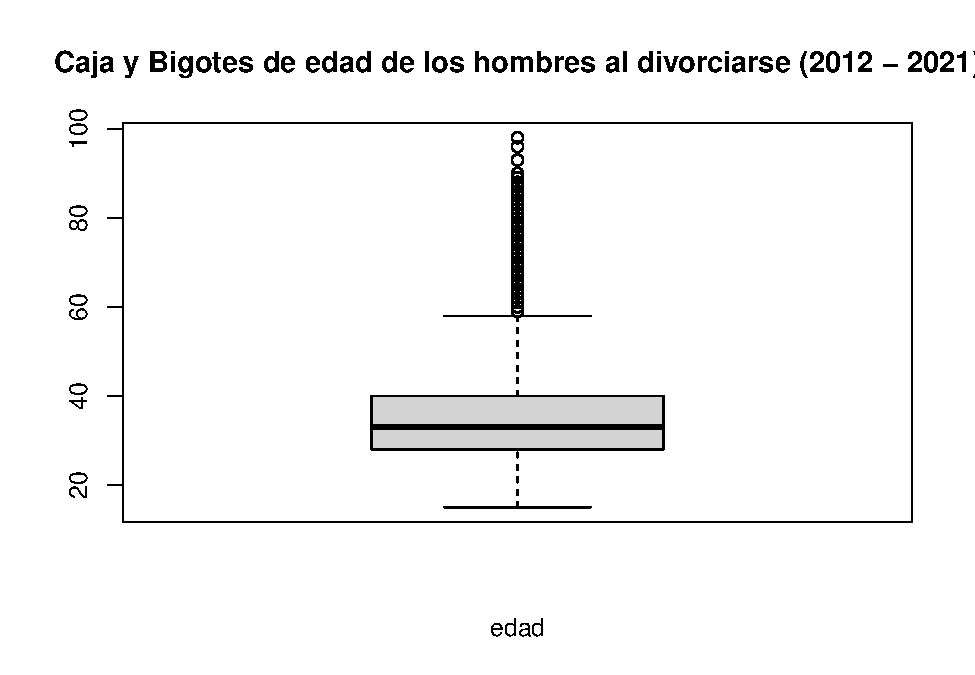
\includegraphics{Proyecto_files/figure-latex/normalBoxEdadHombre-1.pdf}

\hypertarget{diagrama-qqnormal}{%
\subsubsection{Diagrama qqnormal}\label{diagrama-qqnormal}}

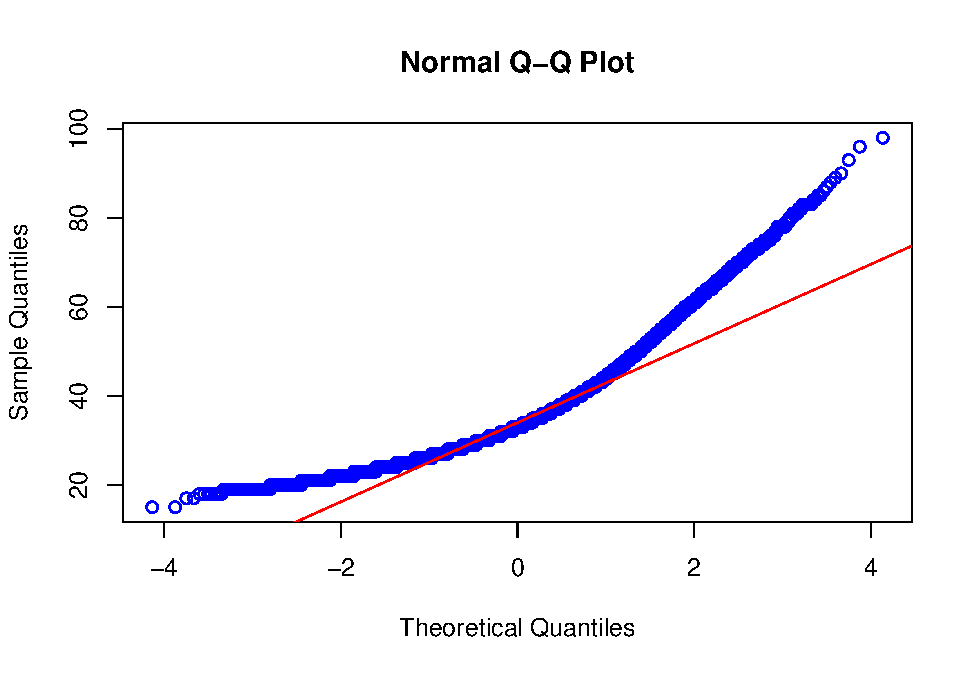
\includegraphics{Proyecto_files/figure-latex/normalQQEdadHombre-1.pdf}

\hypertarget{registros-de-edad-de-mujeres}{%
\subsection{Registros de edad de
mujeres}\label{registros-de-edad-de-mujeres}}

\hypertarget{prueba-de-normalidad-para-la-edad-de-la-mujer}{%
\subsubsection{Prueba de normalidad para la edad de la
mujer:}\label{prueba-de-normalidad-para-la-edad-de-la-mujer}}

\begin{verbatim}
## Don't know how to automatically pick scale for object of type
## <haven_labelled/vctrs_vctr/double>. Defaulting to continuous.
## `stat_bin()` using `bins = 30`. Pick better value with `binwidth`.
\end{verbatim}

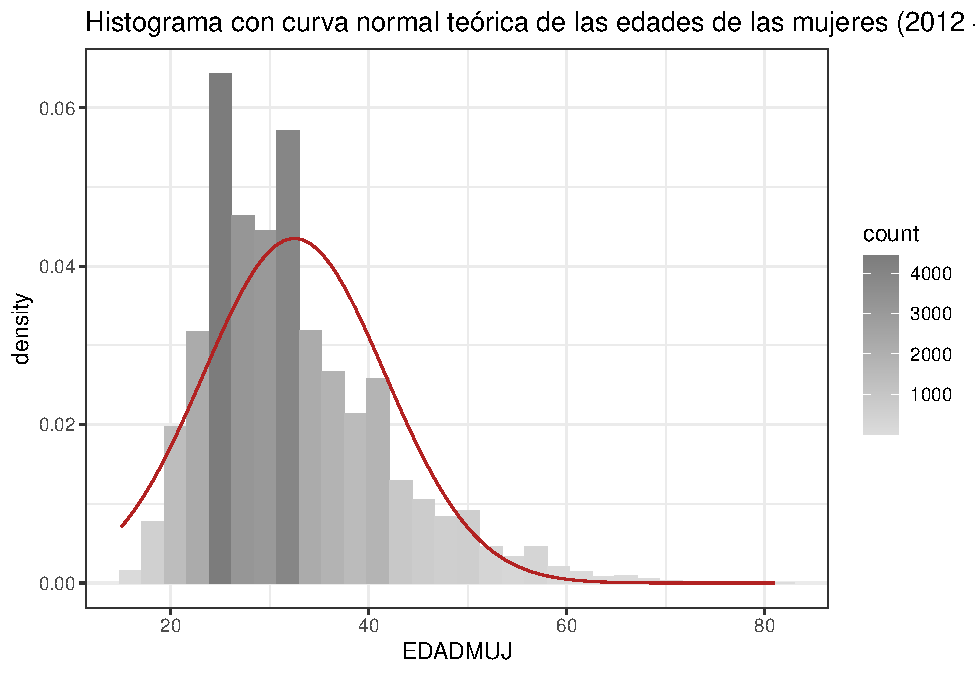
\includegraphics{Proyecto_files/figure-latex/normalHistEdadMuje-1.pdf}

\hypertarget{diagrama-de-caja-y-bigotes-1}{%
\subsubsection{Diagrama de caja y
bigotes}\label{diagrama-de-caja-y-bigotes-1}}

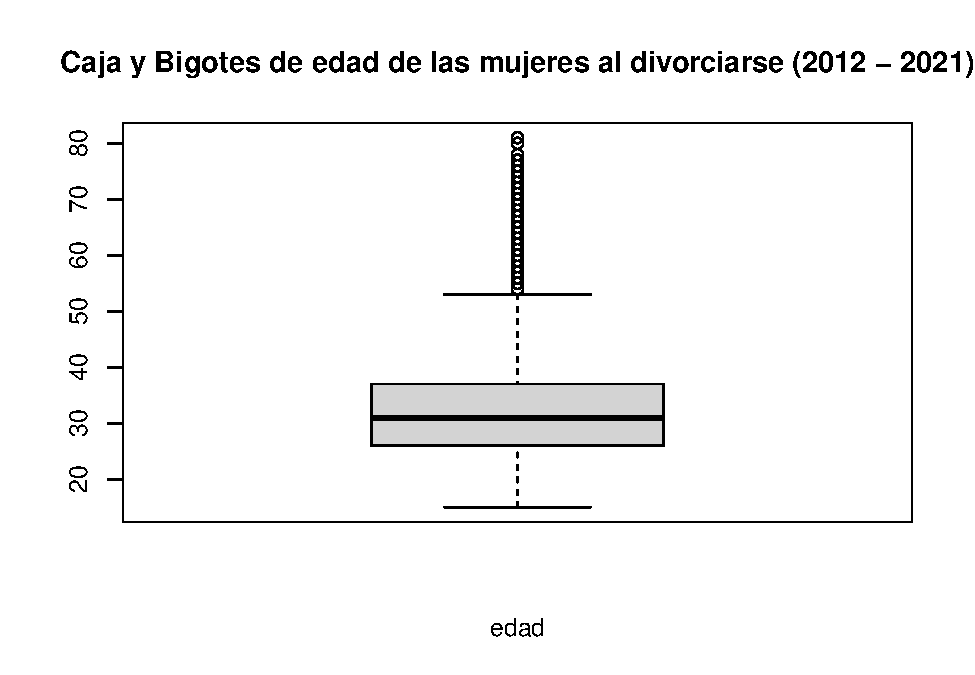
\includegraphics{Proyecto_files/figure-latex/normalBoxEdadMujer-1.pdf}

\hypertarget{diagrama-qqnormal-1}{%
\subsubsection{Diagrama qqnormal}\label{diagrama-qqnormal-1}}

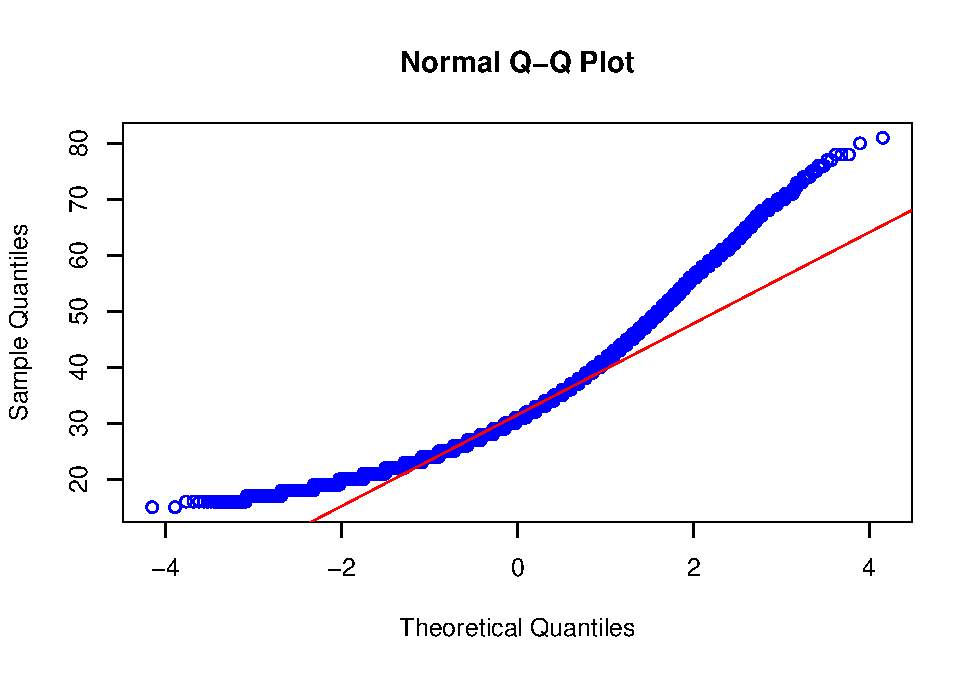
\includegraphics{Proyecto_files/figure-latex/normalQQEdadMujer-1.pdf}

\hypertarget{tabla-de-frecuencias-para-variables-cualitativas}{%
\subsection{Tabla de frecuencias para variables
cualitativas}\label{tabla-de-frecuencias-para-variables-cualitativas}}

\hypertarget{tabla-de-frecuencias-para-el-departamento-de-ocurrencia-y-representaciuxf3n-gruxe1fica}{%
\subsubsection{Tabla de frecuencias para el departamento de ocurrencia y
representación
gráfica}\label{tabla-de-frecuencias-para-el-departamento-de-ocurrencia-y-representaciuxf3n-gruxe1fica}}

\begin{Shaded}
\begin{Highlighting}[]
\NormalTok{D2009 }\OtherTok{\textless{}{-}}\NormalTok{ D2009 }\SpecialCharTok{\%\textgreater{}\%}
  \FunctionTok{mutate\_if}\NormalTok{(is.labelled,}\FunctionTok{list}\NormalTok{(as\_factor))}
\NormalTok{D2010 }\OtherTok{\textless{}{-}}\NormalTok{ D2010 }\SpecialCharTok{\%\textgreater{}\%}
  \FunctionTok{mutate\_if}\NormalTok{(is.labelled,}\FunctionTok{list}\NormalTok{(as\_factor))}
\NormalTok{D2011 }\OtherTok{\textless{}{-}}\NormalTok{ D2011 }\SpecialCharTok{\%\textgreater{}\%}
  \FunctionTok{mutate\_if}\NormalTok{(is.labelled,}\FunctionTok{list}\NormalTok{(as\_factor))}
\NormalTok{D2012 }\OtherTok{\textless{}{-}}\NormalTok{ D2012 }\SpecialCharTok{\%\textgreater{}\%}
  \FunctionTok{mutate\_if}\NormalTok{(is.labelled,}\FunctionTok{list}\NormalTok{(as\_factor))}
\NormalTok{D2013 }\OtherTok{\textless{}{-}}\NormalTok{ D2013 }\SpecialCharTok{\%\textgreater{}\%}
  \FunctionTok{mutate\_if}\NormalTok{(is.labelled,}\FunctionTok{list}\NormalTok{(as\_factor))}
\NormalTok{D2014 }\OtherTok{\textless{}{-}}\NormalTok{ D2014 }\SpecialCharTok{\%\textgreater{}\%}
  \FunctionTok{mutate\_if}\NormalTok{(is.labelled,}\FunctionTok{list}\NormalTok{(as\_factor))}
\NormalTok{D2015 }\OtherTok{\textless{}{-}}\NormalTok{ D2015 }\SpecialCharTok{\%\textgreater{}\%}
  \FunctionTok{mutate\_if}\NormalTok{(is.labelled,}\FunctionTok{list}\NormalTok{(as\_factor))}
\NormalTok{D2016 }\OtherTok{\textless{}{-}}\NormalTok{ D2016 }\SpecialCharTok{\%\textgreater{}\%}
  \FunctionTok{mutate\_if}\NormalTok{(is.labelled,}\FunctionTok{list}\NormalTok{(as\_factor))}
\NormalTok{D2017 }\OtherTok{\textless{}{-}}\NormalTok{ D2017 }\SpecialCharTok{\%\textgreater{}\%}
  \FunctionTok{mutate\_if}\NormalTok{(is.labelled,}\FunctionTok{list}\NormalTok{(as\_factor))}
\NormalTok{D2018 }\OtherTok{\textless{}{-}}\NormalTok{ D2018 }\SpecialCharTok{\%\textgreater{}\%}
  \FunctionTok{mutate\_if}\NormalTok{(is.labelled,}\FunctionTok{list}\NormalTok{(as\_factor))}
\NormalTok{D2019 }\OtherTok{\textless{}{-}}\NormalTok{ D2019 }\SpecialCharTok{\%\textgreater{}\%}
  \FunctionTok{mutate\_if}\NormalTok{(is.labelled,}\FunctionTok{list}\NormalTok{(as\_factor))}
\NormalTok{D2020 }\OtherTok{\textless{}{-}}\NormalTok{ D2020 }\SpecialCharTok{\%\textgreater{}\%}
  \FunctionTok{mutate\_if}\NormalTok{(is.labelled,}\FunctionTok{list}\NormalTok{(as\_factor))}
\NormalTok{D2021 }\OtherTok{\textless{}{-}}\NormalTok{ D2021 }\SpecialCharTok{\%\textgreater{}\%}
  \FunctionTok{mutate\_if}\NormalTok{(is.labelled,}\FunctionTok{list}\NormalTok{(as\_factor))}

\NormalTok{divorciosLabels }\OtherTok{\textless{}{-}} \FunctionTok{bind\_rows}\NormalTok{( D2012, D2013, D2014, D2015, D2016, D2017, D2018, D2019, D2020, D2021)}
\end{Highlighting}
\end{Shaded}

\begin{verbatim}
## 
##      Guatemala    El Progreso   Sacatepequez  Chimaltenango      Escuintla 
##          10008            554            482            815           1418 
##     Santa Rosa         Solola    Totonicapan Quetzaltenango  Suchitepequez 
##            898            312            404           2751            705 
##     Retalhuleu     San Marcos  Huehuetenango         Quiche   Baja Verapaz 
##            912           1455           1107            635            645 
##   Alta Verapaz          Peten         Izabal         Zacapa     Chiquimula 
##            892            579            978            762            798 
##         Jalapa        Jutiapa   Sacatepéquez         Sololá    Totonicapán 
##            604           1474            162             91            171 
##  Suchitepéquez         Quiché          Petén 
##            267            274            225
\end{verbatim}

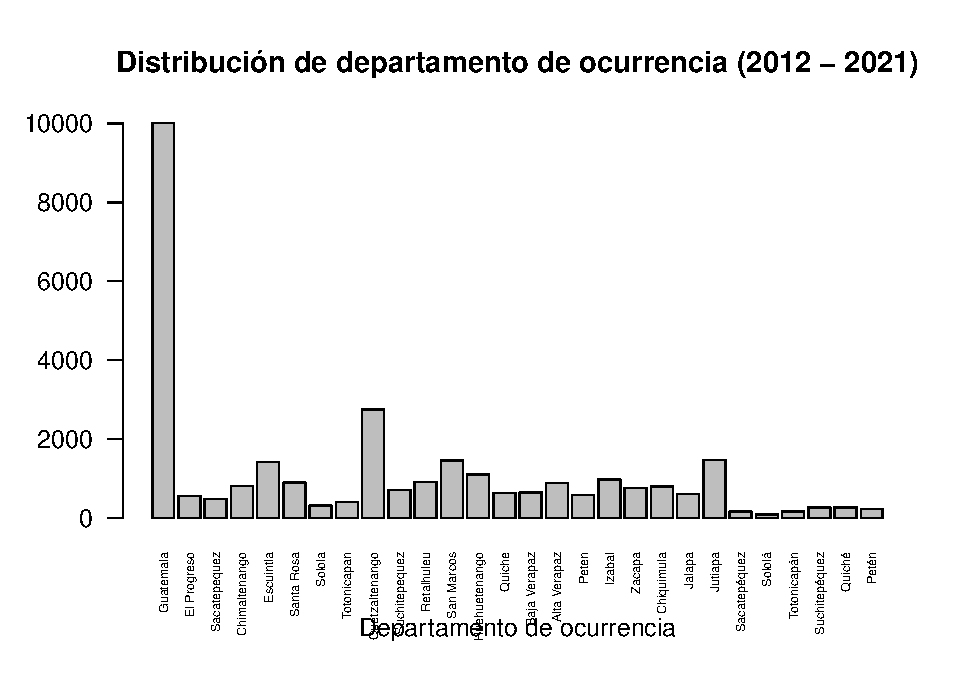
\includegraphics{Proyecto_files/figure-latex/frecuenciaDepartamento-1.pdf}

\hypertarget{tabla-de-frecuencias-para-el-municipio-de-ocurrencia}{%
\subsubsection{Tabla de frecuencias para el municipio de
ocurrencia}\label{tabla-de-frecuencias-para-el-municipio-de-ocurrencia}}

\begin{verbatim}
## 
##                   Guatemala       Santa Catarina Pinula 
##                        6367                         239 
##             San José Pinula          San José del Golfo 
##                         176                          34 
##                    Palencia                   Chinautla 
##                          79                         199 
##           San Pedro Ayampuc                       Mixco 
##                          95                         779 
##      San Pedro Sacatepéquez       San Juan Sacatepéquez 
##                         185                         131 
##                San Raymundo                 Chuarrancho 
##                          91                          19 
##                   Fraijanes                   Amatitlán 
##                          82                         356 
##                 Villa Nueva               Villa Canales 
##                         749                         314 
##                      Petapa                  Guastatoya 
##                         231                         206 
##                     Morazán   San Agustín Acasaguastlán 
##                          29                          58 
## San Cristóbal Acasaguastlán                   El Jícaro 
##                          16                          53 
##                     Sansare                    Sanarate 
##                          33                         107 
##          San Antonio la Paz           Antigua Guatemala 
##                          52                         262 
##                 Jocotenango                    Pastores 
##                          62                          19 
##                    Sumpango       Santo Domingo Xenacoj 
##                          18                           7 
##       Santiago Sacatepéquez  San Bartolomé Milpas Altas 
##                          30                          12 
##      San Lucas Sacatepéquez    Santa Lucía Milpas Altas 
##                          81                          41 
##      Magdalena Milpas Altas        Santa María de Jesús 
##                          19                           5 
##                Ciudad Vieja           San Miguel Dueñas 
##                          35                          15 
##                  Alotenango San Antonio Aguas Calientes 
##                          12                          21 
##     Santa Catarina Barahona               Chimaltenango 
##                           5                         296 
##            San José Poaquil      San Martín Jilotepeque 
##                          18                          47 
##                    Comalapa              Santa Apolonia 
##                          40                           8 
##            Tecpán Guatemala                      Patzún 
##                          90                          53 
##                     Pochuta                    Patzicía 
##                           4                          45 
##          Santa Cruz Balanyá                  Acatenango 
##                          14                          19 
##                    Yepocapa           San Andrés Itzapa 
##                          10                          40 
##                    Parramos                    Zaragoza 
##                          25                          69 
##                    El Tejar                   Escuintla 
##                          37                         524 
##   Santa Lucía Cotzumalguapa               La Democracia 
##                         170                         105 
##                   Siquinalá                     Masagua 
##                          32                          28 
##                   Tiquisate                   La Gomera 
##                         156                          72 
##                 Guanagazapa                    San José 
##                          16                         174 
##                      Iztapa                       Palín 
##                          46                          84 
##          San Vicente Pacaya            Nueva Concepción 
##                          22                          89 
##                     Cuilapa                   Barberena 
##                         182                         156 
##          Santa Rosa de Lima                    Casillas 
##                          47                          40 
##       San Rafael las Flores                    Oratorio 
##                          15                          37 
##            San Juan Tecuaco               Chiquimulilla 
##                          11                         134 
##                     Taxisco        Santa María Ixhuatán 
##                          49                          33 
##                  Guazacapán          Santa Cruz Naranjo 
##                          61                          33 
##          Pueblo Nuevo Viñas            Nueva Santa Rosa 
##                          35                          65 
##                      Sololá            San José Chacayá 
##                         158                           1 
##      Santa María Visitación         Santa Lucía Utatlán 
##                           0                          30 
##                     Nahualá   Santa Catarina Ixtahuacán 
##                          34                          19 
##       Santa Clara la Laguna                  Concepción 
##                          13                           3 
##        San Andrés Semetabaj                  Panajachel 
##                           5                          52 
##       Santa Catarina Palopó          San Antonio Palopó 
##                           4                           7 
##           San Lucas Tolimán        Santa Cruz la Laguna 
##                          31                           5 
##         San Pablo la Laguna        San Marcos la Laguna 
##                           1                           0 
##          San Juan la Laguna         San Pedro la Laguna 
##                          14                          11 
##            Santiago Atitlán                 Totonicapán 
##                          15                         290 
##   San Cristóbal Totonicapán       San Francisco el Alto 
##                          39                          53 
##            San Andrés Xecul                Momostenango 
##                          29                         111 
##      Santa María Chiquimula      Santa Lucía la Reforma 
##                          25                          12 
##                 San Bartolo              Quetzaltenango 
##                          16                        1166 
##                     Salcajá                 Olintepeque 
##                         131                          67 
##             San Carlos Sija                     Sibilia 
##                          57                          16 
##                    Cabricán                      Cajolá 
##                          17                           6 
##          San Miguel Siguilá                  Ostuncalco 
##                           9                          77 
##                   San Mateo    Concepción Chiquirichapa 
##                          20                          30 
##     San Martín Sacatepéquez                   Almolonga 
##                          36                          29 
##                      Cantel                      Huitán 
##                         121                          14 
##                       Zunil                     Colomba 
##                          51                          87 
##      San Francisco la Unión                   El Palmar 
##                          10                          38 
##                  Coatepeque                      Génova 
##                         501                         113 
##           Flores Costa Cuca                La Esperanza 
##                          58                          79 
##      Palestina de los Altos                 Mazatenango 
##                          18                         382 
##                 Cuyotenango    San Francisco Zapotitlán 
##                          92                          67 
##              San Bernardino           San José el Idolo 
##                          57                          11 
## Santo Domingo Suchitepéquez                 San Lorenzo 
##                          15                          28 
##                     Samayac         San Pablo Jocopilas 
##                          44                          23 
##   San Antonio Suchitepéquez            San Miguel Panán 
##                          60                           4 
##                 San Gabriel                    Chicacao 
##                          12                          38 
##                     Patulul               Santa Bárbara 
##                          28                          24 
##           San Juan Bautista        Santo Tomás la Unión 
##                           6                          22 
##                    Zunilito                Pueblo Nuevo 
##                          17                          29 
##                   Río Bravo                  Retalhuleu 
##                          37                         484 
##               San Sebastián            Santa Cruz Muluá 
##                          79                          27 
##       San Martín Zapotitlán                  San Felipe 
##                          29                          46 
##       San Andrés Villa Seca                  Champerico 
##                          75                          78 
##            Nuevo San Carlos                  El Asintal 
##                          50                          44 
##                  San Marcos    San Antonio Sacatepéquez 
##                         167                          20 
##                Comitancillo       San Miguel Ixtahuacán 
##                          12                           9 
##          Concepción Tutuapa                      Tacaná 
##                          13                          21 
##                     Sibinal                   Tajumulco 
##                           3                           8 
##                     Tejutla San Rafael Pié de la Cuesta 
##                          57                          44 
##              Nuevo Progreso                 El Tumbador 
##                          43                          42 
##                    El Rodeo                   Malacatán 
##                          11                         232 
##                    Catarina                      Ayutla 
##                          35                         151 
##                        Ocós                   San Pablo 
##                         105                          58 
##                  El Quetzal                  La Reforma 
##                          71                          29 
##                    Pajapita                   Ixchiguán 
##                          49                          36 
##           San José Ojetenán         San Cristóbal Cucho 
##                           5                          47 
##                    Sipacapa       Esquipulas Palo Gordo 
##                           9                           8 
##                  Río Blanco               Huehuetenango 
##                          26                         516 
##                    Chiantla               Malacatancito 
##                          46                          36 
##                      Cuilco                      Nentón 
##                          24                          12 
##             San Pedro Necta                Jacaltenango 
##                          16                          23 
##                      Soloma                  Ixtahuacán 
##                          44                          23 
##                 La Libertad           San Miguel Acatán 
##                         108                           7 
## San Rafael la Independencia     Todos Santos Cuchumatán 
##                           4                          37 
##             San Juan Atitán               Santa Eulalia 
##                          14                          15 
##           San Mateo Ixtatán                 Colotenango 
##                           2                          14 
## San Sebastián Huehuetenango                    Tectitán 
##                           7                           4 
##           Concepción Huista              San Juan Ixcoy 
##                           7                           9 
##          San Antonio Huista        San Sebastián Coatán 
##                          16                          37 
##                    Barillas                   Aguacatán 
##                          33                          21 
##           San Rafael Petzal           San Gaspar Ixchil 
##                           5                           2 
##      Santiago Chimaltenango            Santa Ana Huista 
##                           5                           4 
##              Unión Cantinil       Santa Cruz del Quiché 
##                           2                         280 
##                      Chiché                    Chinique 
##                          16                          23 
##                    Zacualpa                      Chajul 
##                          33                           8 
##            Chichicastenango                     Patzité 
##                          79                           5 
##      San Antonio Ilotenango         San Pedro Jocopilas 
##                          22                          12 
##                       Cunén             San Juan Cotzal 
##                          33                          10 
##                     Joyabaj                       Nebaj 
##                         105                          73 
##        San Andrés Sajcabajá                    Uspantán 
##                          12                          37 
##                   Sacapulas   San Bartolomé Jocotenango 
##                          41                           5 
##                     Canillá                    Chicamán 
##                          23                          18 
##                       Ixcán                    Pachalum 
##                          44                          30 
##                      Salamá           San Miguel Chicaj 
##                         304                          23 
##                     Rabinal                     Cubulco 
##                          84                          73 
##                    Granados                     El Chol 
##                          28                          29 
##                San Jerónimo                     Purulhá 
##                          80                          24 
##                       Cobán          Santa Cruz Verapaz 
##                         453                          32 
##       San Cristóbal Verapaz                      Tactic 
##                          68                          48 
##                      Tamahú                      Tucurú 
##                           6                           6 
##                      Panzós                      Senahú 
##                           7                          13 
##            San Pedro Carchá           San Juan Chamelco 
##                          97                          51 
##                     Lanquín                     Cahabón 
##                           6                           5 
##                      Chisec                      Chahal 
##                          32                           5 
## Fray Bartolomé de las Casas     Santa Catalina la Tinta 
##                          48                          11 
##                     Raxruhá                      Flores 
##                           4                         108 
##                  San Benito                  San Andrés 
##                         208                          41 
##               San Francisco                   Santa Ana 
##                          37                          18 
##                     Dolores                    San Luis 
##                          49                          27 
##                    Sayaxché           Melchor de Mencos 
##                          36                          37 
##                      Poptún                  Las Cruces 
##                         129                          12 
##              Puerto Barrios                  Livingston 
##                         617                          58 
##                    El Estor                     Morales 
##                          22                         197 
##                  Los Amates                      Zacapa 
##                          84                         395 
##                  Estanzuela                   Río Hondo 
##                          56                          85 
##                      Gualán                   Teculután 
##                         107                          32 
##                   Usumatlán                     Cabañas 
##                          13                          18 
##                   San Diego                    La Unión 
##                          27                          15 
##                       Huité                  Chiquimula 
##                           9                         308 
##           San José La Arada             San Juan Ermita 
##                          27                          21 
##                     Jocotán                     Camotán 
##                          31                          15 
##                       Olopa                  Esquipulas 
##                          24                         116 
##        Concepción Las Minas              Quetzaltepeque 
##                          78                          53 
##                 San Jacinto                       Ipala 
##                          10                         115 
##                      Jalapa            San Pedro Pinula 
##                         387                          29 
##        San Luis Jilotepeque        San Manuel Chaparrón 
##                          31                          19 
##         San Carlos Alzatate                      Monjas 
##                          10                          99 
##             Mataquescuintla                     Jutiapa 
##                          29                         500 
##                 El Progreso         Santa Catarina Mita 
##                         152                          91 
##                 Agua Blanca               Asunción Mita 
##                          78                         160 
##                Yupiltepeque                 Atescatempa 
##                          23                          49 
##                       Jerez                 El Adelanto 
##                          13                           9 
##                  Zapotitlán                      Comapa 
##                          13                          39 
##                  Jalpatagua                    Conguaco 
##                         114                           9 
##                      Moyuta                      Pasaco 
##                          91                           5 
##           San José Acatempa                     Quesada 
##                          81                          47 
##         San José La Maquina                   La Blanca 
##                           0                           8 
##                     El Chal                   San Jorge 
##                           6                           5 
##                    Sipacate         San José la Maquina 
##                           0                           4 
##                     Petatán                  Extranjero 
##                           0                           0 
##                    Ignorado 
##                           0
\end{verbatim}

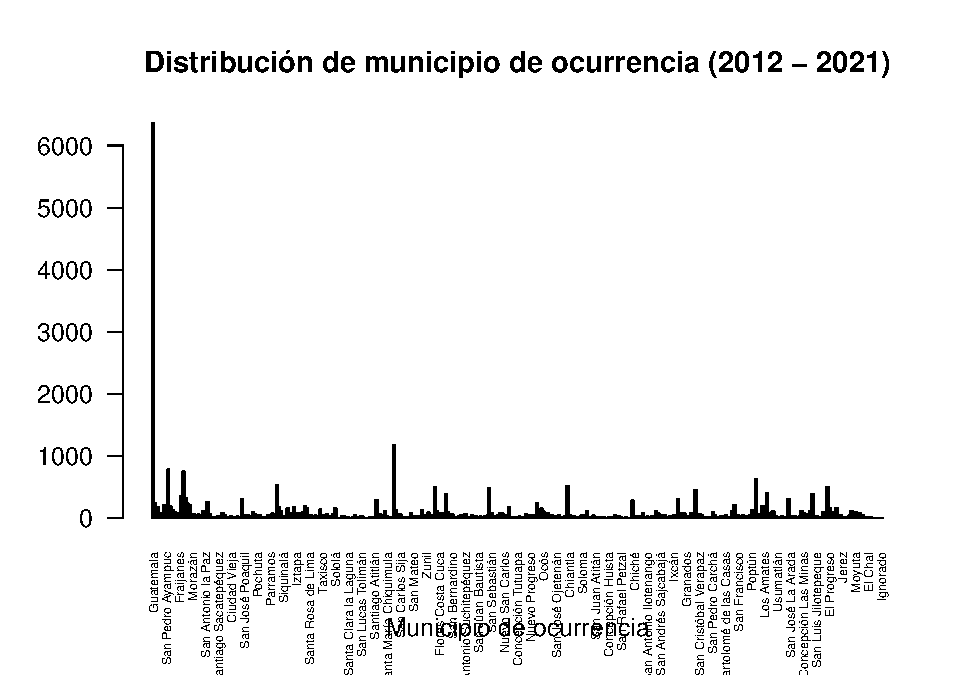
\includegraphics{Proyecto_files/figure-latex/frecuenciaMunicipio-1.pdf}

\hypertarget{tabla-de-frecuencias-para-la-escolaridad-del-hombre}{%
\subsubsection{Tabla de frecuencias para la escolaridad del
hombre}\label{tabla-de-frecuencias-para-la-escolaridad-del-hombre}}

\begin{verbatim}
## 
##       Ninguna      Primaria        Básico Diversificado Universitario 
##           318          4846          3138         10566          3149 
##      Ignorado       Ninguno     Postgrado        Básica    Post Grado 
##          5275          2752             7           280            47 
##     Doctorado 
##             0
\end{verbatim}

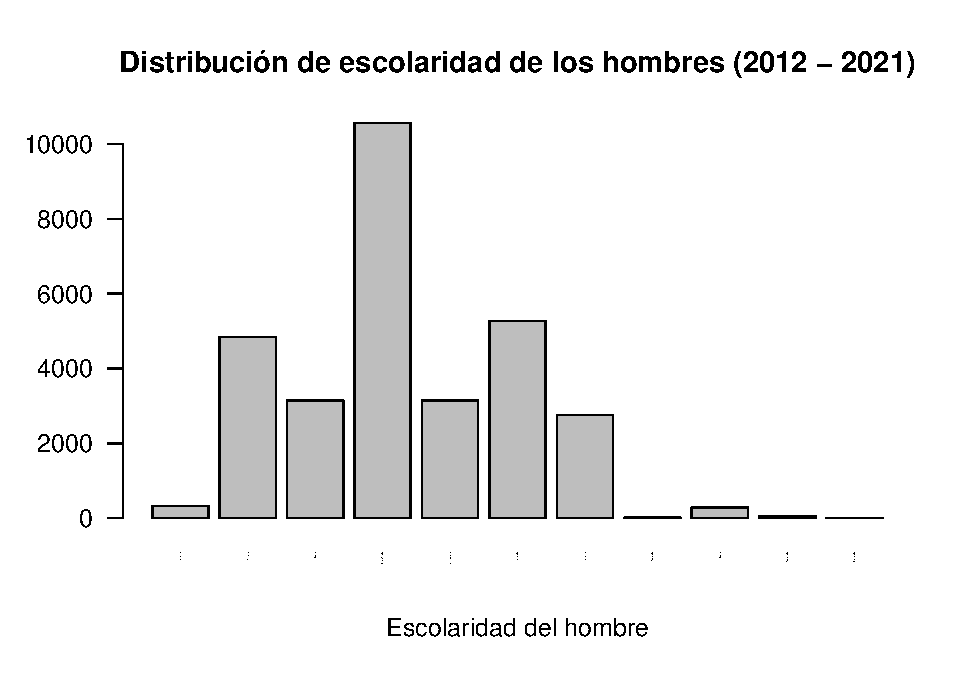
\includegraphics{Proyecto_files/figure-latex/frecuenciaEscolaridadHombre-1.pdf}

\hypertarget{tabla-de-frecuencias-para-la-escolaridad-de-la-mujer}{%
\subsubsection{Tabla de frecuencias para la escolaridad de la
Mujer}\label{tabla-de-frecuencias-para-la-escolaridad-de-la-mujer}}

\begin{verbatim}
## 
##       Ninguna      Primaria        Básico Diversificado Universitario 
##           347          5118          3439         11462          3082 
##      Ignorado       Ninguno     Postgrado        Básica    Post Grado 
##          3534          3074             4           289            29 
##     Doctorado 
##             0
\end{verbatim}

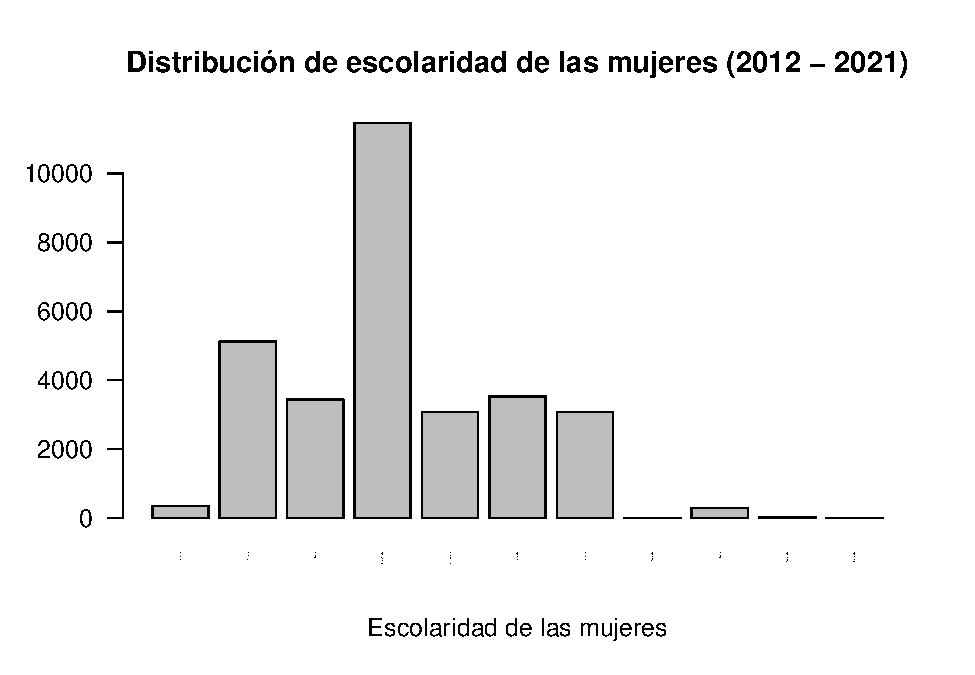
\includegraphics{Proyecto_files/figure-latex/frecuenciaEscolaridadMujer-1.pdf}

\hypertarget{tabla-de-frecuencias-para-el-grupo-uxe9tnico-del-hombre}{%
\subsubsection{Tabla de frecuencias para el grupo étnico del
hombre}\label{tabla-de-frecuencias-para-el-grupo-uxe9tnico-del-hombre}}

\begin{verbatim}
## 
##         Garífuna         Ignorado         Indigena Ladino / Mestizo 
##               18             6141              182            19355 
##             Maya      No indigena             Otro            Xinka 
##             3564              820              293                5
\end{verbatim}

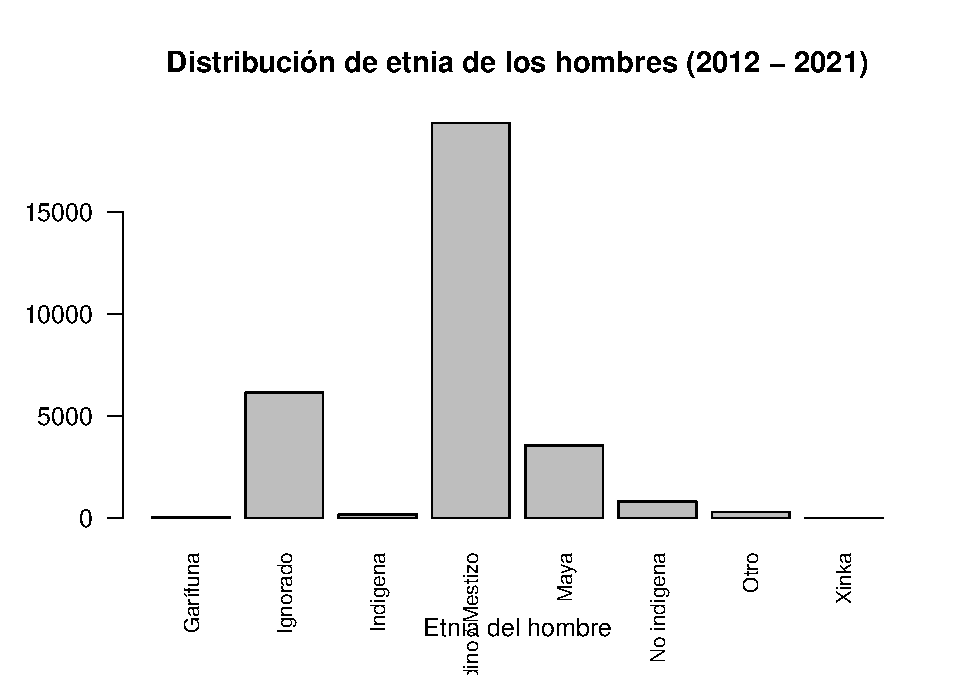
\includegraphics{Proyecto_files/figure-latex/frecuenciaEtniaHombre-1.pdf}

\hypertarget{tabla-de-frecuencias-para-el-grupo-uxe9tnico-de-la-mujer}{%
\subsubsection{Tabla de frecuencias para el grupo étnico de la
mujer}\label{tabla-de-frecuencias-para-el-grupo-uxe9tnico-de-la-mujer}}

\begin{verbatim}
## 
##         Garífuna         Ignorado         Indigena Ladino / Mestizo 
##               21             4740              192            20671 
##             Maya      No indigena             Otro            Xinka 
##             3401              987              363                3
\end{verbatim}

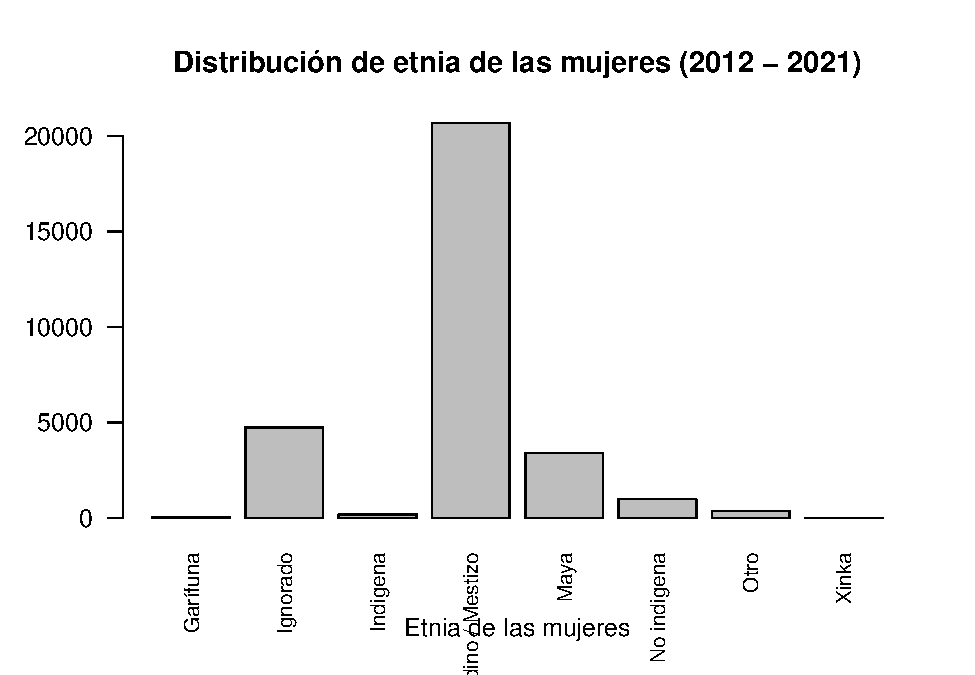
\includegraphics{Proyecto_files/figure-latex/frecuenciaEtniaMujer-1.pdf}

\hypertarget{correlacion-entre-edades-de-los-cuxf3nyuges}{%
\subsection{Correlacion entre edades de los
cónyuges}\label{correlacion-entre-edades-de-los-cuxf3nyuges}}

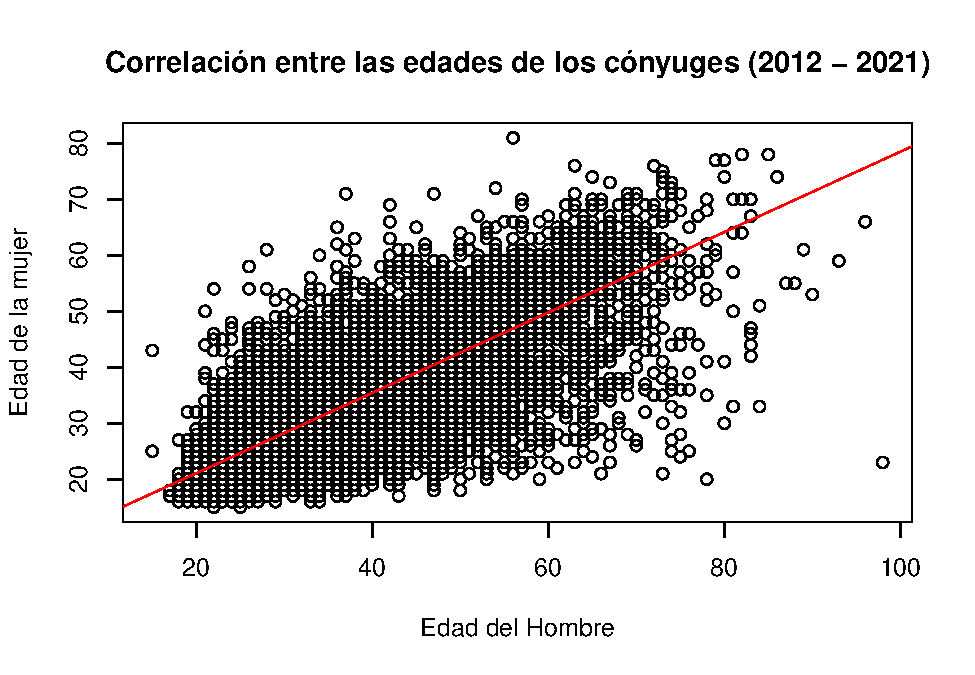
\includegraphics{Proyecto_files/figure-latex/CorrelacionEdades-1.pdf}

\hypertarget{ocupacion-en-hombre-2009-2021}{%
\subsection{Ocupacion en Hombre
2009-2021}\label{ocupacion-en-hombre-2009-2021}}

\hypertarget{ocupacion-en-mujeres-2009-2021}{%
\subsection{ocupacion en Mujeres
2009-2021}\label{ocupacion-en-mujeres-2009-2021}}

\hypertarget{clustering}{%
\subsection{Clustering}\label{clustering}}

Haga un agrupamiento (clustering) e interprete los resultados.

\begin{Shaded}
\begin{Highlighting}[]
\NormalTok{divorcios}\SpecialCharTok{$}\NormalTok{AÑOOCU }\OtherTok{\textless{}{-}} \FunctionTok{as.numeric}\NormalTok{(}\FunctionTok{factor}\NormalTok{(divorcios}\SpecialCharTok{$}\NormalTok{AÑOOCU))}
\NormalTok{datosClustering }\OtherTok{\textless{}{-}}\NormalTok{ divorcios[,}\FunctionTok{c}\NormalTok{(}\StringTok{"AÑOREG"}\NormalTok{,}\StringTok{"EDADHOM"}\NormalTok{,}\StringTok{"EDADMUJ"}\NormalTok{,}\StringTok{"AÑOOCU"}\NormalTok{)]}
\NormalTok{data\_omit }\OtherTok{\textless{}{-}} \FunctionTok{na.omit}\NormalTok{(datosClustering) }
\FunctionTok{summary}\NormalTok{(datosClustering)}
\end{Highlighting}
\end{Shaded}

\begin{verbatim}
##      AÑOREG        EDADHOM         EDADMUJ          AÑOOCU     
##  Min.   :2012   Min.   : 15.0   Min.   :15.00   Min.   :1.000  
##  1st Qu.:2015   1st Qu.: 29.0   1st Qu.:26.00   1st Qu.:3.000  
##  Median :2018   Median : 34.0   Median :31.00   Median :5.000  
##  Mean   :2018   Mean   :106.8   Mean   :32.49   Mean   :4.482  
##  3rd Qu.:2020   3rd Qu.: 42.0   3rd Qu.:37.00   3rd Qu.:7.000  
##  Max.   :2022   Max.   :999.0   Max.   :81.00   Max.   :7.000  
##                                                 NA's   :6027
\end{verbatim}

\begin{verbatim}
## Warning: did not converge in 10 iterations
\end{verbatim}

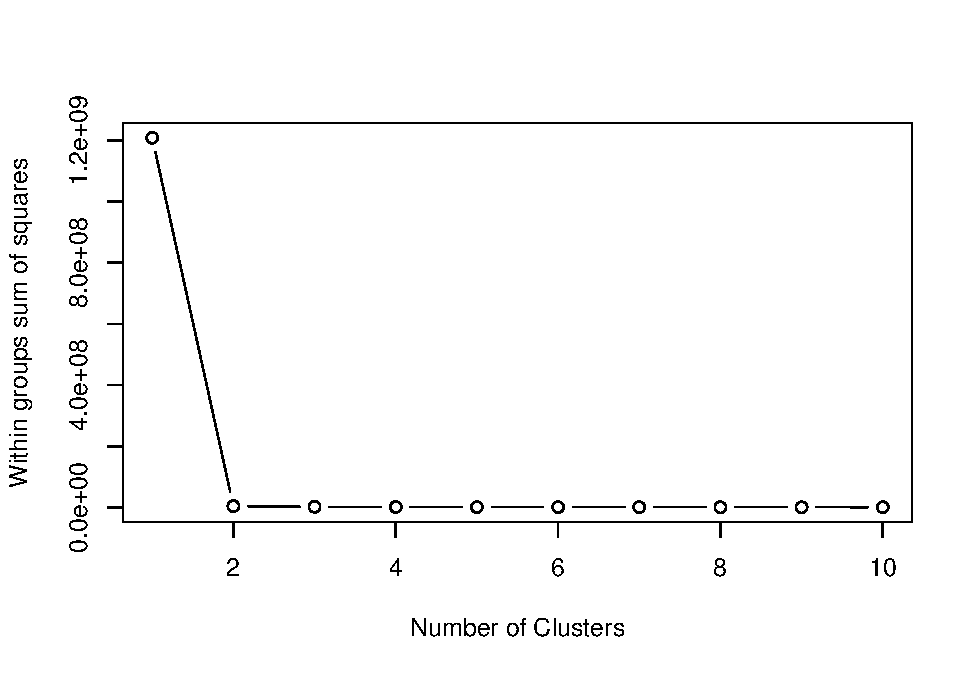
\includegraphics{Proyecto_files/figure-latex/cantClusters-1.pdf}

\hypertarget{edad-mujeres-y-hombres-en-divorcio-entre-2009-2021-por-medio-de-k-means}{%
\subsection{Edad mujeres y hombres en divorcio entre 2009-2021 por medio
de
k-means}\label{edad-mujeres-y-hombres-en-divorcio-entre-2009-2021-por-medio-de-k-means}}

\hypertarget{agrupamiento-por-medio-de-k-means}{%
\subsection{Agrupamiento por medio de
k-means}\label{agrupamiento-por-medio-de-k-means}}

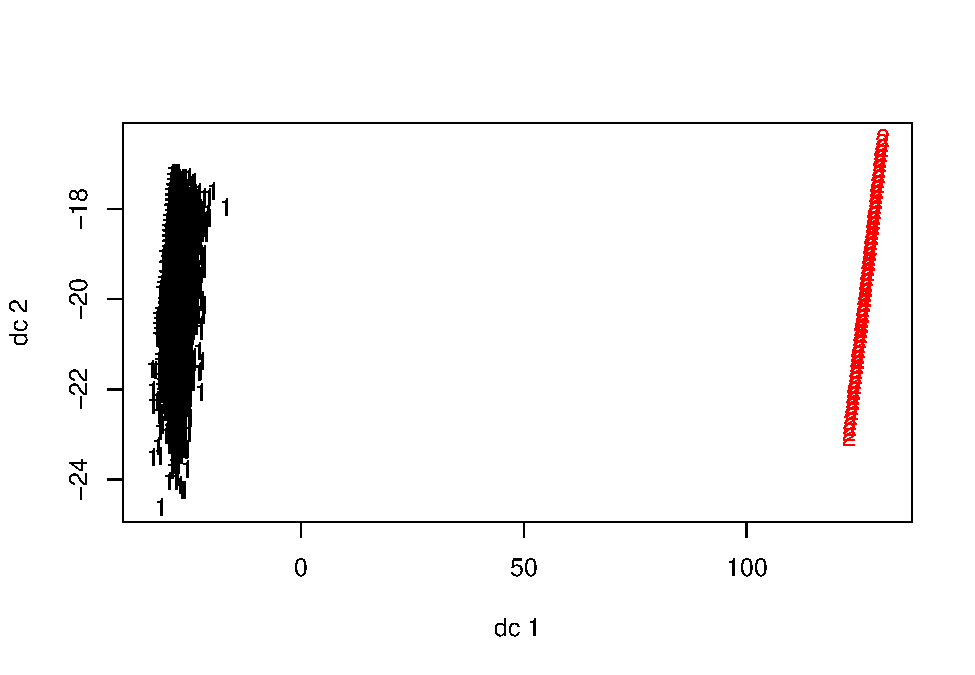
\includegraphics{Proyecto_files/figure-latex/kmeans2-1.pdf}

\hypertarget{mixture-of-gaussians}{%
\subsection{Mixture of gaussians}\label{mixture-of-gaussians}}

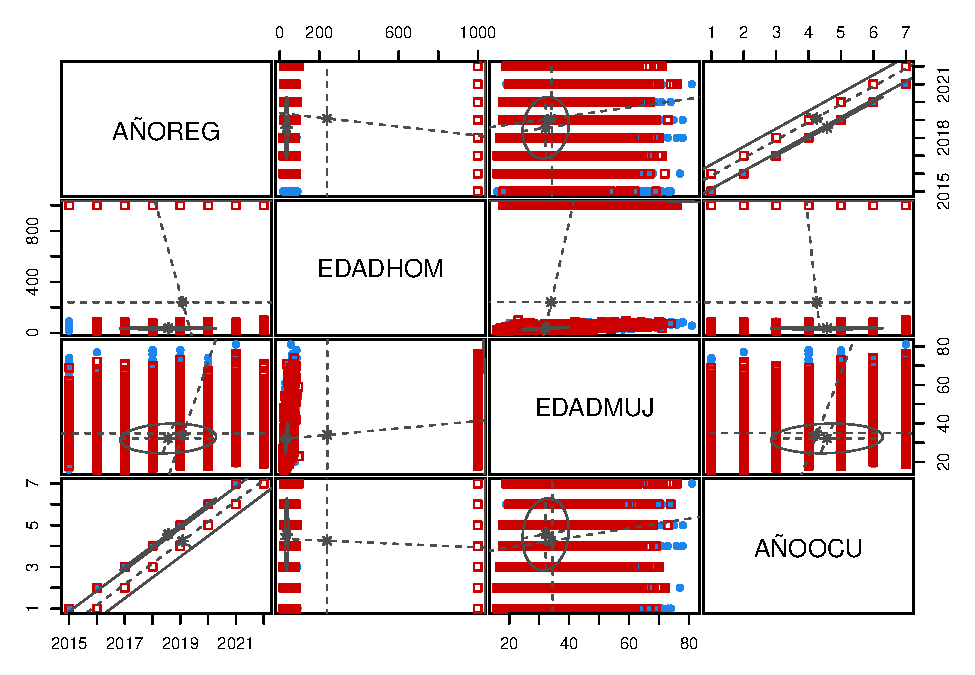
\includegraphics{Proyecto_files/figure-latex/gaussians-1.pdf}

\hypertarget{fuzzy-c-means}{%
\subsection{Fuzzy C-means}\label{fuzzy-c-means}}

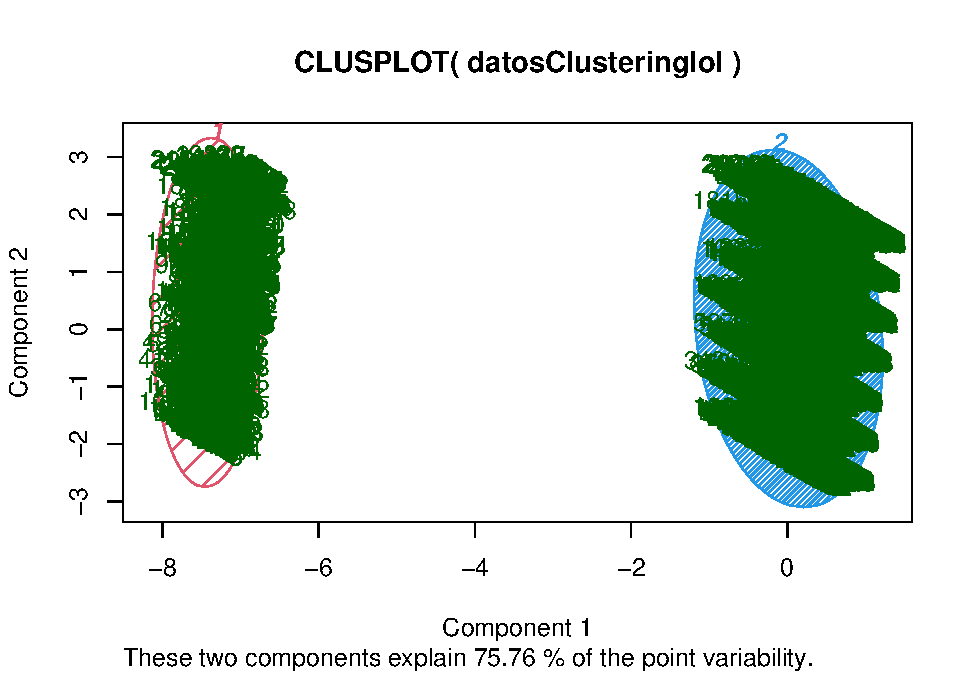
\includegraphics{Proyecto_files/figure-latex/fuzzy2-1.pdf}
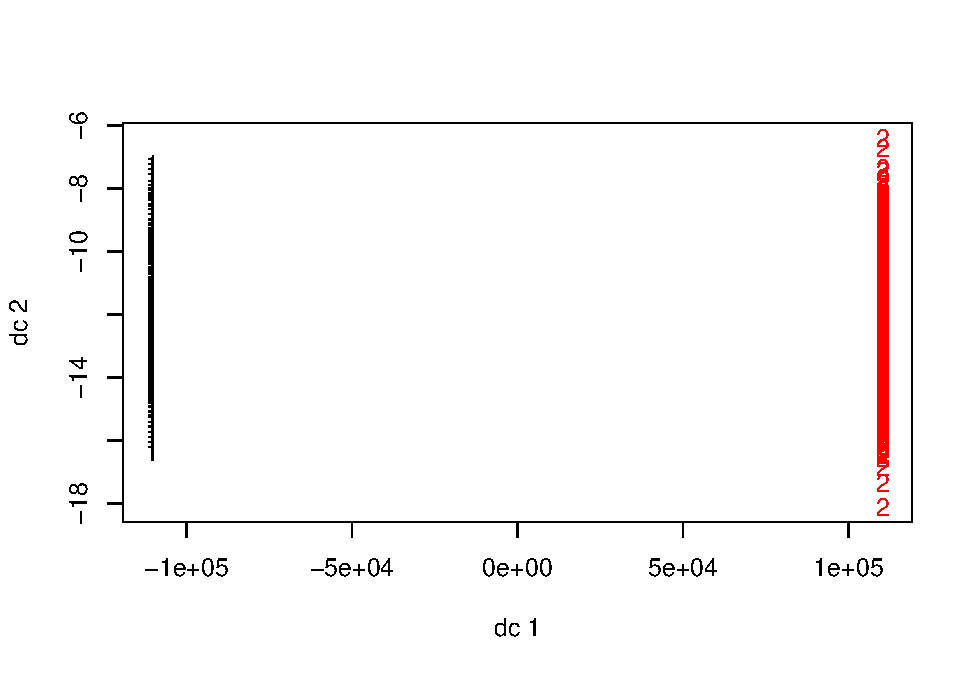
\includegraphics{Proyecto_files/figure-latex/fuzzy2-2.pdf}

\begin{verbatim}
##      AÑOREG        EDADHOM         EDADMUJ          AÑOOCU          grupo  
##  Min.   :2015   Min.   :18.00   Min.   :16.00   Min.   :1.000   Min.   :1  
##  1st Qu.:2017   1st Qu.:28.00   1st Qu.:26.00   1st Qu.:3.000   1st Qu.:1  
##  Median :2019   Median :33.00   Median :30.00   Median :5.000   Median :1  
##  Mean   :2019   Mean   :35.34   Mean   :32.17   Mean   :4.516   Mean   :1  
##  3rd Qu.:2021   3rd Qu.:40.00   3rd Qu.:37.00   3rd Qu.:7.000   3rd Qu.:1  
##  Max.   :2022   Max.   :98.00   Max.   :81.00   Max.   :7.000   Max.   :1
\end{verbatim}

\begin{verbatim}
##      AÑOREG        EDADHOM       EDADMUJ          AÑOOCU          grupo  
##  Min.   :2015   Min.   :999   Min.   :18.00   Min.   :1.000   Min.   :2  
##  1st Qu.:2016   1st Qu.:999   1st Qu.:34.00   1st Qu.:2.000   1st Qu.:2  
##  Median :2018   Median :999   Median :40.00   Median :4.000   Median :2  
##  Mean   :2018   Mean   :999   Mean   :40.99   Mean   :3.921   Mean   :2  
##  3rd Qu.:2020   3rd Qu.:999   3rd Qu.:46.75   3rd Qu.:6.000   3rd Qu.:2  
##  Max.   :2022   Max.   :999   Max.   :76.00   Max.   :7.000   Max.   :2
\end{verbatim}

\begin{verbatim}
##      AÑOREG        EDADHOM         EDADMUJ          AÑOOCU          grupo  
##  Min.   :2015   Min.   :18.00   Min.   :16.00   Min.   :1.000   Min.   :1  
##  1st Qu.:2017   1st Qu.:28.00   1st Qu.:26.00   1st Qu.:3.000   1st Qu.:1  
##  Median :2019   Median :33.00   Median :30.00   Median :5.000   Median :1  
##  Mean   :2019   Mean   :35.32   Mean   :32.18   Mean   :4.566   Mean   :1  
##  3rd Qu.:2021   3rd Qu.:40.00   3rd Qu.:37.00   3rd Qu.:7.000   3rd Qu.:1  
##  Max.   :2021   Max.   :90.00   Max.   :81.00   Max.   :7.000   Max.   :1  
##      mxGau  
##  Min.   :1  
##  1st Qu.:1  
##  Median :1  
##  Mean   :1  
##  3rd Qu.:1  
##  Max.   :1
\end{verbatim}

\begin{verbatim}
##      AÑOREG        EDADHOM         EDADMUJ          AÑOOCU          grupo      
##  Min.   :2015   Min.   : 18.0   Min.   :16.00   Min.   :1.000   Min.   :1.000  
##  1st Qu.:2017   1st Qu.: 30.0   1st Qu.:27.00   1st Qu.:3.000   1st Qu.:1.000  
##  Median :2019   Median : 36.0   Median :32.00   Median :4.000   Median :1.000  
##  Mean   :2019   Mean   :239.6   Mean   :34.01   Mean   :4.252   Mean   :1.212  
##  3rd Qu.:2021   3rd Qu.: 56.0   3rd Qu.:39.00   3rd Qu.:6.000   3rd Qu.:1.000  
##  Max.   :2022   Max.   :999.0   Max.   :76.00   Max.   :7.000   Max.   :2.000  
##      mxGau  
##  Min.   :2  
##  1st Qu.:2  
##  Median :2  
##  Mean   :2  
##  3rd Qu.:2  
##  Max.   :2
\end{verbatim}

\begin{verbatim}
##      AÑOREG        EDADHOM       EDADMUJ          AÑOOCU          grupo  
##  Min.   :2015   Min.   :999   Min.   :18.00   Min.   :1.000   Min.   :2  
##  1st Qu.:2016   1st Qu.:999   1st Qu.:34.00   1st Qu.:2.000   1st Qu.:2  
##  Median :2018   Median :999   Median :40.00   Median :4.000   Median :2  
##  Mean   :2018   Mean   :999   Mean   :40.99   Mean   :3.921   Mean   :2  
##  3rd Qu.:2020   3rd Qu.:999   3rd Qu.:46.75   3rd Qu.:6.000   3rd Qu.:2  
##  Max.   :2022   Max.   :999   Max.   :76.00   Max.   :7.000   Max.   :2  
##      mxGau      FCGrupos
##  Min.   :2   Min.   :1  
##  1st Qu.:2   1st Qu.:1  
##  Median :2   Median :1  
##  Mean   :2   Mean   :1  
##  3rd Qu.:2   3rd Qu.:1  
##  Max.   :2   Max.   :1
\end{verbatim}

\begin{verbatim}
##      AÑOREG        EDADHOM         EDADMUJ          AÑOOCU          grupo  
##  Min.   :2015   Min.   :18.00   Min.   :16.00   Min.   :1.000   Min.   :1  
##  1st Qu.:2017   1st Qu.:28.00   1st Qu.:26.00   1st Qu.:3.000   1st Qu.:1  
##  Median :2019   Median :33.00   Median :30.00   Median :5.000   Median :1  
##  Mean   :2019   Mean   :35.34   Mean   :32.17   Mean   :4.516   Mean   :1  
##  3rd Qu.:2021   3rd Qu.:40.00   3rd Qu.:37.00   3rd Qu.:7.000   3rd Qu.:1  
##  Max.   :2022   Max.   :98.00   Max.   :81.00   Max.   :7.000   Max.   :1  
##      mxGau          FCGrupos
##  Min.   :1.000   Min.   :2  
##  1st Qu.:1.000   1st Qu.:2  
##  Median :1.000   Median :2  
##  Mean   :1.222   Mean   :2  
##  3rd Qu.:1.000   3rd Qu.:2  
##  Max.   :2.000   Max.   :2
\end{verbatim}

\hypertarget{evaluaciuxf3n-de-la-tendencia-de-agrupamiento}{%
\subsection{Evaluación de la tendencia de
agrupamiento:}\label{evaluaciuxf3n-de-la-tendencia-de-agrupamiento}}

\hypertarget{en-hombres}{%
\subsubsection{En hombres}\label{en-hombres}}

\includegraphics{Proyecto_files/figure-latex/Evaluacion de la tendencia de agrupamiento:cluster jerarquico-1.pdf}

\hypertarget{en-mujeres}{%
\subsubsection{En mujeres}\label{en-mujeres}}

\includegraphics{Proyecto_files/figure-latex/elegir los algoritmos de agrupación apropiados-1.pdf}

\end{document}
